\chapter{Propuesta de arquitectura inteligente y softwarizada enfocada al IIoT}
\label{ch:datadriven}

En este capítulo se presentan las contribuciones principales asociadas al segundo bloque de objetivos de la Tesis, centradas en el diseño de una arquitectura \gls{iiot} inteligente y softwarizada. La propuesta se articula sobre marcos de orquestación unificados que integran salidas de inferencia en tiempo real basadas en \gls{ai}/\gls{ml}, obtenidas de la telemetría de los sensores, con el fin de habilitar reconfiguraciones dinámicas de red, reubicación eficiente de servicios y mantenimiento preventivo.\\
\\
Esta línea de trabajo tuvo su origen en el proyecto 6G-DATADRIVEN‑02 (en colaboración con la Universidad Carlos III de Madrid)~\cite{6g-datadriven-arch}, donde se establecieron los fundamentos conceptuales de la arquitectura. Posteriormente, se desarrolló una primera prueba de concepto (PoC), presentada en la conferencia ICIN 2025~\cite{carrascal2025softwarized}, que mostró la viabilidad de la aproximación propuesta mediante un producto mínimo viable basado en virtualización clásica. Más adelante, durante la estancia doctoral en la Universidad de Milán-Bicocca, la arquitectura evolucionó hacia un despliegue orientado a microservicios y contenedores, integrando mecanismos de inferencia en el plano de control y ampliando los conjuntos de datos utilizados para evaluar la capacidad de autorreconfiguración en escenarios \gls{iiot} realistas. Estas pruebas incluyeron evaluaciones de rendimiento y resiliencia, que confirmaron la validez, flexibilidad y adaptabilidad de la arquitectura propuesta. Fruto de este trabajo se ha derivado una publicación~\cite{Carrascal2025milan}, actualmente en proceso de revisión, que consolida esta línea de investigación como un paso clave hacia el diseño de ecosistemas industriales inteligentes, distribuidos y softwarizados.

\section{Introducción}

La evolución del \gls{iiot} ha puesto de manifiesto la necesidad de arquitecturas capaces de integrar inteligencia distribuida, baja latencia y mecanismos de adaptación dinámica en escenarios industriales cada vez más complejos y heterogéneos. Como se revisó en el Capítulo~\ref{ch:sota}, Sección~\ref{subsec:iiotarch}, las soluciones existentes presentan avances relevantes en el uso de \textit{edge/fog computing} y arquitecturas softwarizadas, pero persisten retos fundamentales relacionados con la escalabilidad, la interoperabilidad y la ausencia de implementaciones abiertas y reproducibles que materialicen los principios propuestos.\\
\\
En este contexto, se plantea una arquitectura \textit{data-driven} que opera a lo largo del continuo \textit{cloud–edge–\gls{iiot}}, diseñada para cerrar la brecha entre propuestas conceptuales y despliegues prácticos. La arquitectura se fundamenta en tres ejes principales: (i) la adopción de microservicios contenerizados y orquestados mediante plataformas \textit{cloud}-nativas, que facilitan elasticidad y despliegue modular; (ii) la integración de un plano de control dinámico que aprovecha inferencias en tiempo real de modelos \gls{ml} para activar reconfiguraciones de red, reubicación de servicios y mantenimiento preventivo; y (iii) el empleo de estándares abiertos y marcos interoperables que habilitan su aplicación en escenarios heterogéneos y de alta densidad de nodos. La propuesta se valida a través de pruebas de concepto que han evolucionado desde entornos basados en virtualización clásica hasta despliegues orientados a microservicios gestionados por Kubernetes, incluyendo evaluaciones con múltiples conjuntos de datos y condiciones representativas de escenarios industriales. Los resultados obtenidos demuestran reducciones significativas de latencia, mejoras en la capacidad de respuesta ante condiciones cambiantes y una mayor resiliencia frente a cargas variables de sensores y servicios.\\
\\
Con ello, la arquitectura \textit{data-driven} contribuye a los objetivos de la Tesis al proporcionar una base práctica y reproducible para el diseño de sistemas \gls{iiot} inteligentes, escalables y transparentes, alineados con las visiones de redes distribuidas e impulsadas por datos en el horizonte del \gls{6g}.

\section{Descripción de la arquitectura}
\label{sec:system}

Nuestra arquitectura se construye sobre el marco general de diseño establecido por el proyecto 6G-\allowbreak DATADRIVEN-02~\cite{6g-datadriven-arch}, inicialmente validado a través de la prueba de concepto~\cite{carrascal2025softwarized}. La arquitectura está diseñada para operar de forma nativa y continua a lo largo de todo el continuo \textit{cloud–edge–\gls{iiot}}. El objetivo principal es aprovechar los datos generados por dispositivos industriales heterogéneos (sensores, actuadores y \glspl{gw}) para habilitar procesamiento localizado con tiempos de respuesta mínimos, así como adaptabilidad y reconfiguración de red, además de una coordinación colaborativa entre múltiples instalaciones y una visión global unificada en la nube. La Figura~\ref{fig:draft_sysarch} muestra la arquitectura general del sistema.\\
\\
La figura ilustra una arquitectura multinivel que habilita despliegues de \gls{iiot} a lo largo del continuo \textit{cloud–edge–factory}. En el nivel inferior, la arquitectura comienza en el \textit{factory floor}, donde los dispositivos IIoT (p.ej., brazos robóticos, sistemas de transporte, terminales de control) se conectan mediante \glspl{gw}. Estos \glspl{gw} recopilan flujos de datos provenientes de sensores y actuadores dentro de las fábricas y los transmiten hacia niveles superiores. Tecnologías de acceso de red como 5G, 6G o WiMAX interconectan estas pasarelas (\glspl{gw}) con una plataforma en el borde (en el \textit{edge}), donde un módulo de control supervisa el enrutamiento del tráfico y la orquestación. Los flujos de datos se almacenan de manera selectiva en las bases de datos (\glspl{db}) distribuidas a nivel de \textit{edge}. Este plano de control en el \textit{edge} gestiona dinámicamente múltiples plantas industriales, optimizando el uso de la red y el rendimiento de las aplicaciones \gls{iiot}. En niveles superiores, la plataforma en la nube aloja módulos \gls{faas} que incorporan canalizaciones de servicios de inferencias \gls{ai}/\gls{ml}. Estos módulos consumen datos desde las \glspl{db} del \textit{edge} para ejecutar analíticas predictivas, como detección de fallos o control adaptativo, reduciendo la latencia y la sobrecarga computacional en la planta. Los módulos de monitorización proporcionan observabilidad y permiten a los usuarios recibir retroalimentación en tiempo real a lo largo de todos los niveles.

\begin{figure}[ht!]
    \centering
    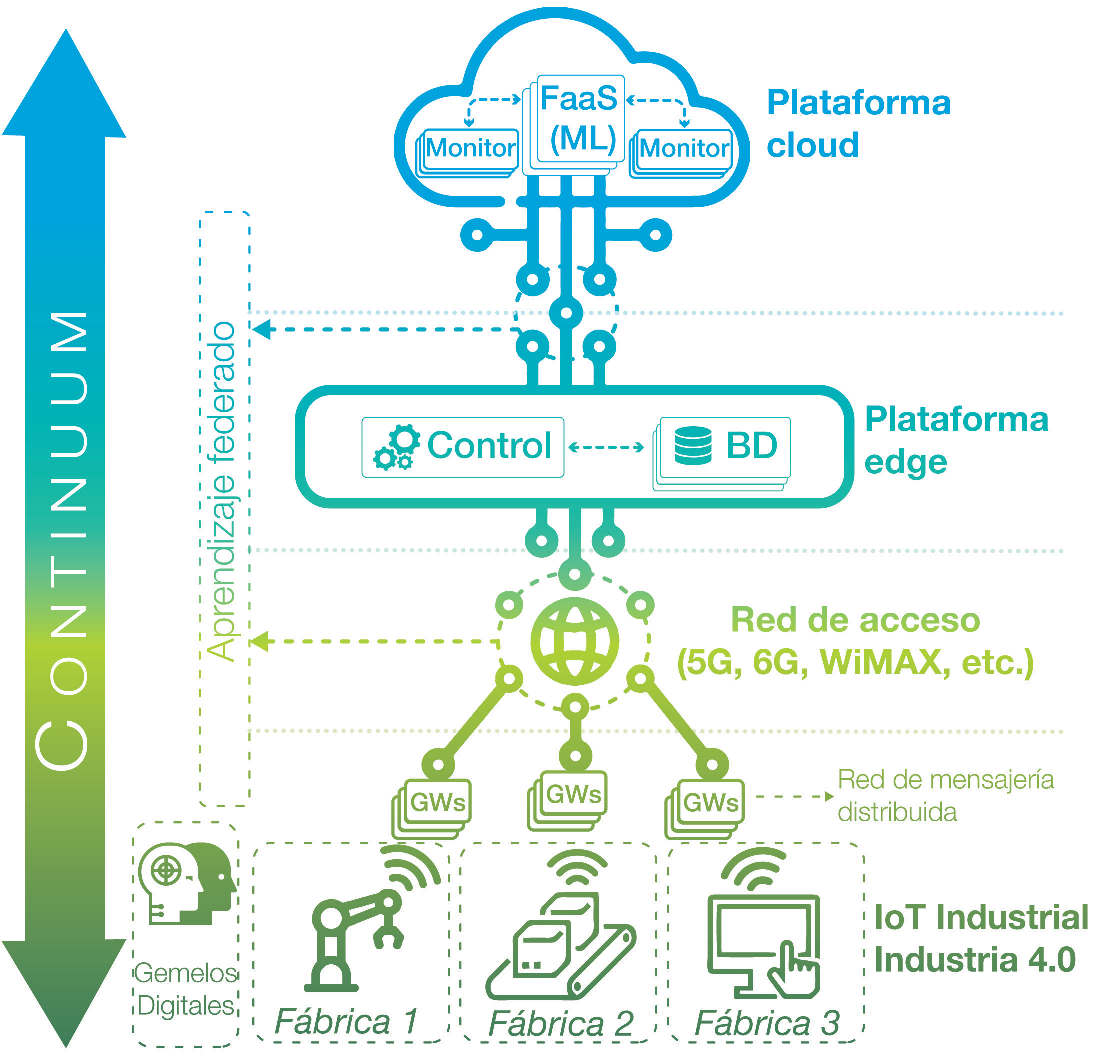
\includegraphics[width=0.9\textwidth]{fig/08_datadriven/datadriven_01.pdf}
    \caption{Visión general de la arquitectura del sistema.}
    \label{fig:draft_sysarch}
\end{figure}

La arquitectura soporta \textit{federated learning} (\gls{fl}), donde el conocimiento derivado de una planta puede contribuir a modelos globales, garantizando inteligencia compartida entre instalaciones. La plataforma en la nube consolida los resultados de todas las fábricas, proporcionando una visión operacional unificada y habilitando que el módulo de control en el \textit{edge} aplique políticas globales de ubicación de servicios, enrutamiento y asignación de recursos. Además, la arquitectura incorpora varios servicios fundamentales para reforzar la resiliencia y la extensibilidad en todos los niveles. Una red distribuida de mensajería desacopla las pasarelas \gls{iiot} de los consumidores, permitiendo que nuevos módulos de inferencia o control se suscriban a los flujos de sensores sin interrumpir los flujos de datos existentes. Cada planta industrial mantiene un gemelo digital local que refleja de manera continua sus activos físicos, y participa en la capa de \textit{federated learning}, mejorando así la precisión de las predicciones. Finalmente, uno de los puntos más importantes es la observabilidad extremo a extremo (mediante registros, métricas y trazas) proporciona visibilidad en todo el continuo, soportando monitorización proactiva y planificación estratégica de largo plazo.\\
\\
En conjunto, esta arquitectura continua, softwarizada y orientada a datos,  habilita:
\begin{itemize}
  \item Reconfiguración automática de redes \gls{iiot} basada en el estado operativo de cada planta.
  \item Procesamiento distribuido y de baja latencia en el borde, garantizando acciones reactivas inmediatas.
  \item Colaboración federada entre fábricas para aprendizaje conjunto y transferencia de conocimiento.
  \item Visión operacional unificada, control global y optimización continua desde la nube y el borde.
\end{itemize} 

\section{Implementación y despliegue de la arquitectura}

En esta sección se detallan la implementación y el despliegue de la arquitectura introducida en la Sección~\ref{sec:system}. Tal y como se señaló previamente, la arquitectura está concebida de manera fundamentalmente orientada a los datos. En consecuencia, la Sección~\ref{subsec:data} comienza con un análisis del conjunto de datos empleado para simular las lecturas de sensores \gls{iiot} en el entorno de la fábrica, junto con los modelos de aprendizaje automático utilizados para tareas de clasificación. Esta subsección se introduce en primer lugar, dado que ciertos aspectos clave basados en datos, como la noción de estado de eficiencia de los sensores y su papel en el desencadenamiento de eventos de reconfiguración de la red, resultan esenciales para comprender la lógica y el comportamiento de los componentes descritos posteriormente.\\
\\
La Sección~\ref{subsec:blocks} describe la implementación de los componentes funcionales básicos de la arquitectura. Finalmente, la Sección~\ref{subsec:k8s} presenta el despliegue basado en Kubernetes, el cual adopta un enfoque orientado a microservicios que garantiza escalabilidad, resiliencia y flexibilidad a lo largo del continuo fábrica–\textit{edge–cloud}.

\subsection{Análisis del conjunto de datos y entrenamiento del modelo de clasificación}
\label{subsec:data}

El funcionamiento de la arquitectura está impulsado por los datos generados a partir de los sensores \gls{iiot}. Ante la falta de acceso a un entorno industrial físico, se recurre a un conjunto de datos \gls{iiot} de acceso público que contiene lecturas temporales de sensores y actuadores. El conjunto de datos seleccionado, disponible en Kaggle~\cite{intelligent_manufacturing_dataset}, es sometido a un análisis estadístico con el fin de extraer las características relevantes, las cuales se utilizan posteriormente para simular el comportamiento de los sensores en el despliegue. A partir de dichas características, se entrena un modelo de clasificación capaz de detectar estados anómalos en los nodos, activando los mecanismos de reconfiguración de red cuando resulte necesario.


\subsubsection{Análisis de conjuntos de datos IIoT}

El conjunto de datos seleccionado incluye mediciones completas en forma de series temporales de procesos industriales. El dataset recopila datos físicos de sensores (temperatura, vibración, consumo energético), indicadores de rendimiento de red (latencia, pérdida de paquetes, eficiencia en la comunicación), así como métricas de producción (tasas de defectos, errores operativos). Dicho conjunto, nos permite evaluar la eficiencia de las máquinas considerando simultáneamente las lecturas de sensores, las condiciones de red y los indicadores de desempeño productivo. La Tabla~\ref{tab:dataset_characteristics} resume las características principales del conjunto de datos.

\begin{table}[ht!]
\centering
\resizebox{\textwidth}{!}{
\begin{tabular}{|p{5cm}|c|p{7.5cm}|}
\hline
\textbf{Característica} & \textbf{Tipo de dato} & \textbf{Descripción} \\
\hline
\texttt{Timestamp}                           & Datetime & Marca temporal de cada lectura. \\
\hline
\texttt{Machine\_ID}                         & Integer   & Identificador único de cada máquina \gls{iiot}. \\
\hline
\texttt{Operation\_Mode}                     & String   & Modo de operación de cada máquina \gls{iiot}. \\
\hline
\texttt{Temperature\_C}                      & Float     & Temperatura (ºC). \\
\hline
\texttt{Vibration\_Hz}                       & Float     & Vibración (Hz). \\
\hline
\texttt{Power\_Consumption\_kW}              & Float     & Consumo energético (kW). \\
\hline
\texttt{Network\_Latency\_ms}                & Float     & Latencia de red (ms). \\
\hline
\texttt{Packet\_Loss\_\%}                    & Float     & Pérdida de paquetes (\%). \\
\hline
\texttt{Quality\_Ctrl\_Defect\_Rate}         & Float     & Tasa de defectos en control de calidad (\%). \\
\hline
\texttt{Prod\_Speed\_units\_per\_hr}         & Float     & Velocidad de producción (unidades/hora). \\
\hline
\texttt{Predict\_Maintenance\_Score}         & Float     & Predicción de mantenimiento (\%). \\
\hline
\texttt{Error\_Rate\_\%}                     & Float     & Tasa de errores (\%). \\
\hline
\texttt{Efficiency\_Status}                  & String   & Clasificación de la eficiencia de fabricación basada en métricas de rendimiento. \\
\hline
\end{tabular}
}
\caption{Características principales del conjunto de datos.}
\label{tab:dataset_characteristics}
\end{table}


El conjunto de datos se ha sometido a un análisis estadístico para extraer las características relevantes, las cuales se emplean posteriormente para emular el comportamiento de los sensores en nuestro despliegue. Un análisis estructural del conjunto de datos, basado en la matriz de correlación (véase la Figura~\ref{fig:variables_correlation}), revela que las características numéricas listadas en la Tabla~\ref{tab:dataset_characteristics} presentan una correlación lineal muy baja entre sí. Esta ausencia de redundancia entre características resulta ventajosa, ya que sugiere que cada característica aporta información distinta y no solapada entre diferentes características del conjunto de datos.

\begin{figure}[ht!]
    \centering
    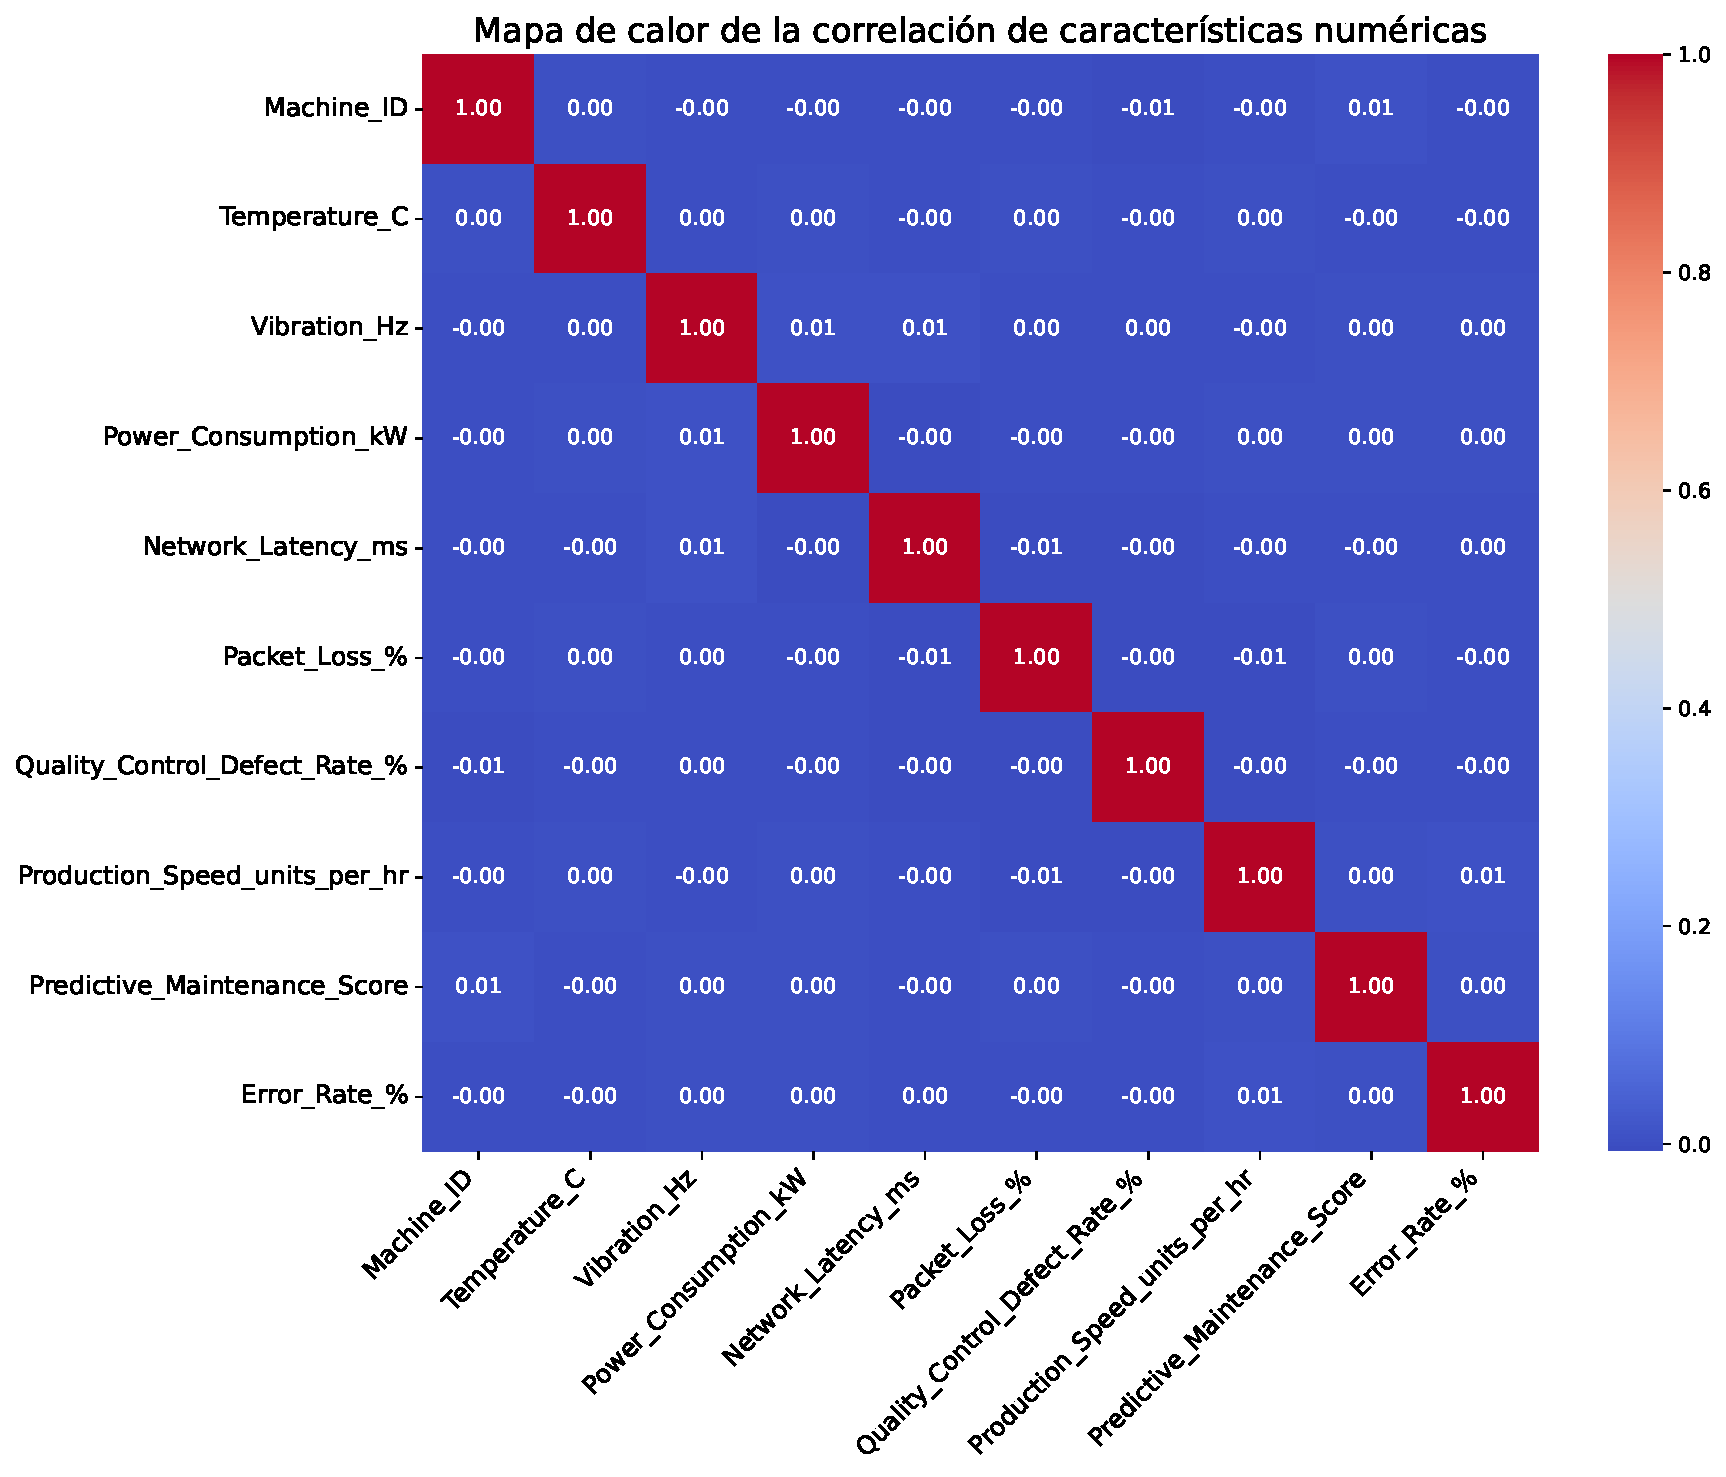
\includegraphics[width=\textwidth]{fig/08_datadriven/datadriven_02.pdf}
    \caption{Mapa de calor de la correlación de las características numéricas del dataset.}
    \label{fig:variables_correlation}
\end{figure}

Un análisis estadístico adicional de las distribuciones de características muestra que todas las variables numéricas siguen una distribución aproximadamente uniforme (véase la Figura~\ref{fig:all_histograms_english}). Este aspecto resulta especialmente relevante para nuestra arquitectura, ya que respalda la extracción de estadísticas descriptivas con el fin de simular datos de sensores realistas en ausencia de hardware físico. \\
\\
En contraste, las variables categóricas, \texttt{Operation\_Mode} y \texttt{Efficiency\_Status}, presentan distribuciones tipo delta, en las que ciertas categorías están notablemente sobrerrepresentadas (como se ilustra en la Figura~\ref{fig:all_histograms_english}). Además, el conjunto de datos exhibe irregularidades temporales, puesto que el atributo \texttt{Month} muestra una fuerte concentración de registros entre los meses de enero, febrero y marzo.


\begin{figure}[ht!]
    \centering
    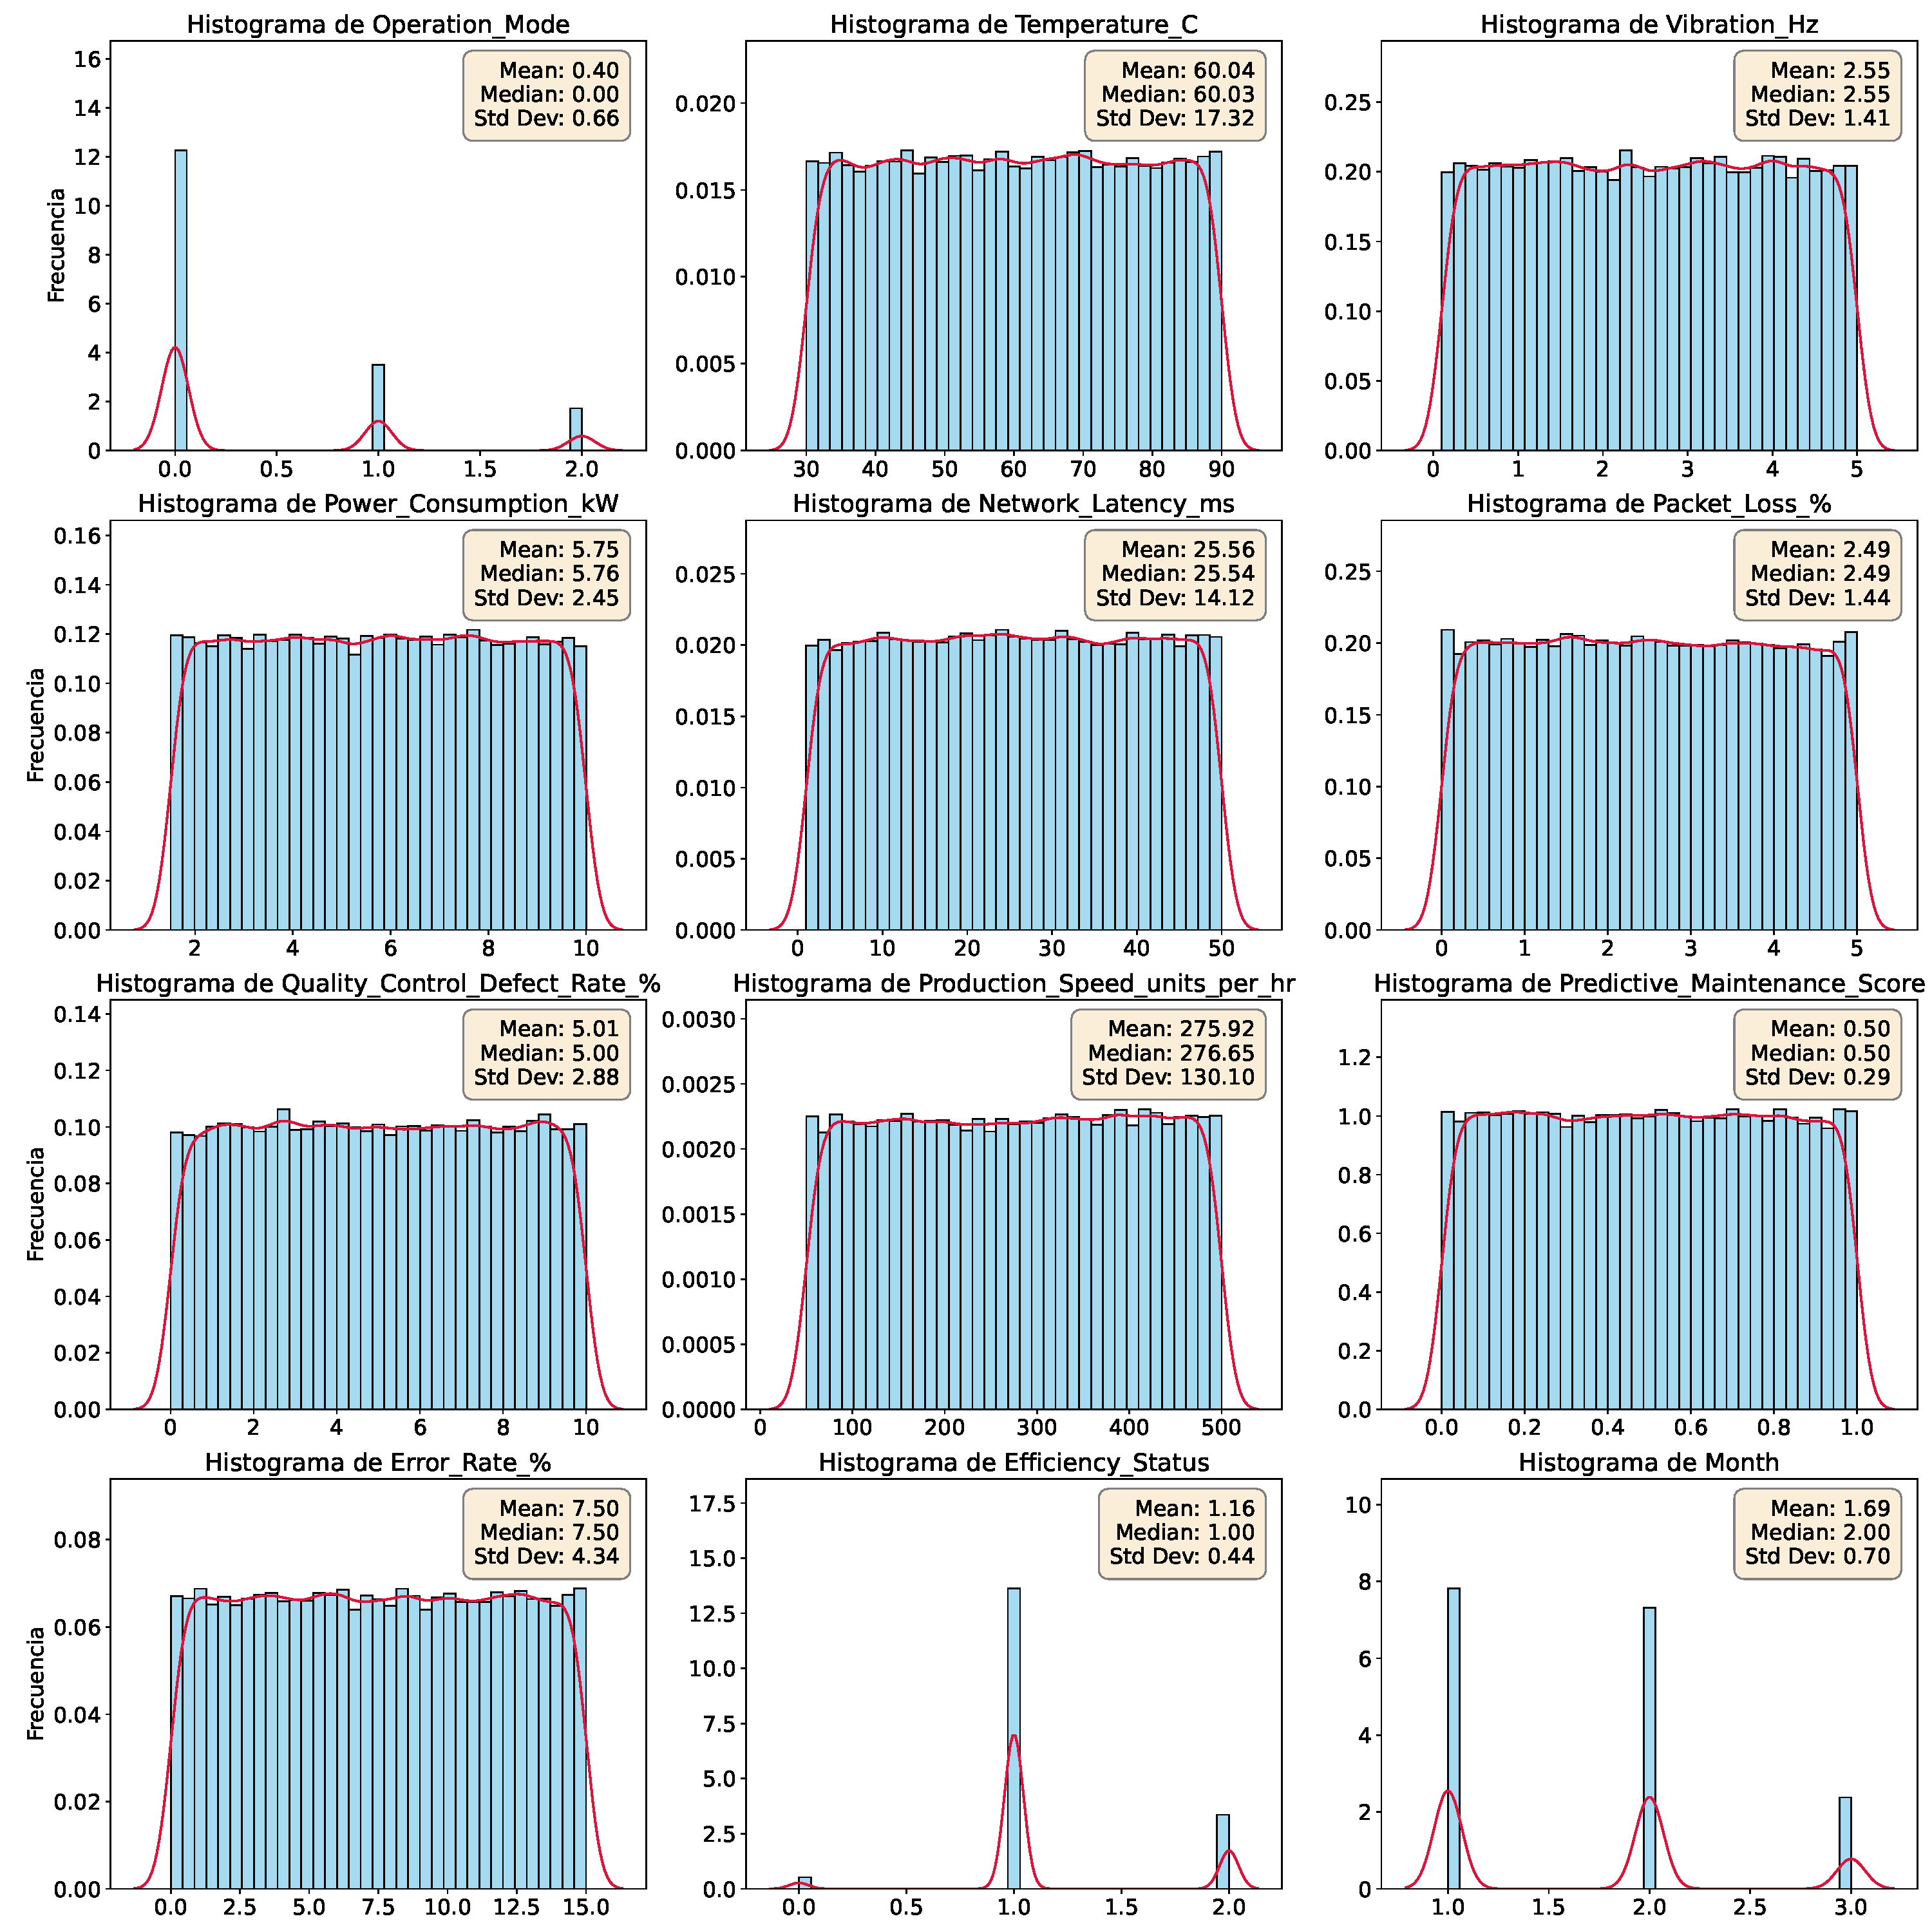
\includegraphics[width=\textwidth]{fig/08_datadriven/datadriven_03.pdf}
    \caption{Histogramas de las distribuciones y estadísticas principales para cada característica del conjunto de datos.}
    \label{fig:all_histograms_english}
\end{figure}

Para lograr una simulación realista de los datos, se analizaron los intervalos de tiempo entre lecturas consecutivas de los sensores. El histograma de estos intervalos, mostrado en la Figura~\ref{fig:interval_time}, revela una distribución sesgada a la derecha, con la mayoría de los intervalos concentrados en valores bajos. Sin embargo, el conjunto de datos también contiene brechas esporádicas de hasta 8,5 horas (aproximadamente 514 minutos o 30.840 segundos). El intervalo de tiempo medio es de aproximadamente 2.998,40 segundos (alrededor de 50 minutos), mientras que la mediana se sitúa en 2.100,00 segundos. La diferencia entre la media y la mediana confirma la prevalencia de intervalos más cortos debido al sesgo de la distribución. Asimismo, la elevada desviación estándar indica una variabilidad considerable en los tiempos de reporte de los sensores. Para fines de implementación, este intervalo medio ha sido normalizado a un intervalo configurable de simulación de 1 segundo, preservando los patrones temporales relativos y permitiendo pruebas en tiempo real de la arquitectura.


\begin{figure}[ht!]
    \centering
    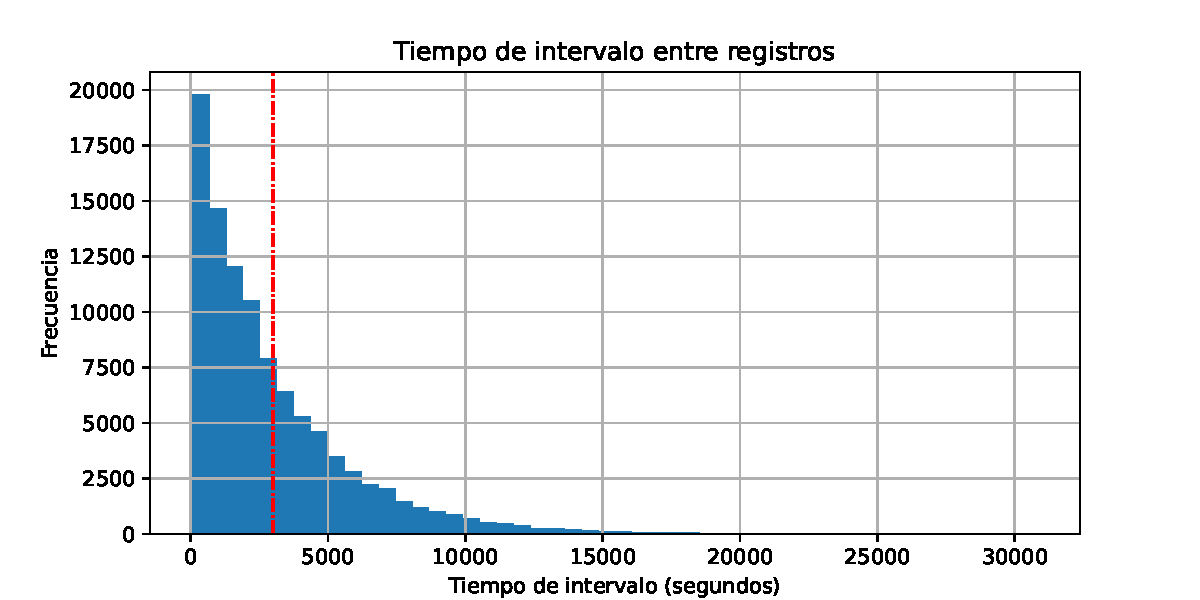
\includegraphics[width=0.85\textwidth]{fig/08_datadriven/datadriven_04.pdf}
    \caption{Intervalo de tiempo en segundos entre las marcas de tiempo de los registros.}
    \label{fig:interval_time}
\end{figure}

\subsubsection{Entrenamiento del modelo de clasificación del estado de eficiencia de los sensores IIoT}
\label{subsubsec:model}

Como se describió en la Sección~\ref{sec:system}, la capa del \textit{cloud} incluye un módulo \gls{faas} encargado de ejecutar funciones de inferencia que determinan si un sensor está operando de manera anómala. Para respaldar esta funcionalidad, se entrenó un modelo de \gls{ml} utilizando el atributo \texttt{Efficiency\_Status} disponible en el conjunto de datos, el cual etiqueta el comportamiento de los sensores en tres clases: baja, media y alta eficiencia. Se seleccionó un clasificador \gls{svm} debido a su alto rendimiento en la tarea. El modelo entrenado alcanzó valores de precisión del 97,5\%, demostrando una elevada capacidad para diferenciar entre los distintos niveles de eficiencia.\\
\\
Aunque podrían haberse explorado modelos adicionales, el enfoque de este trabajo no reside en optimizar el rendimiento de \gls{ml}, sino en diseñar una arquitectura capaz de integrar diversos modelos de \gls{ai}/\gls{ml} según sea necesario para distintos casos de uso.\\
\\
La Figura~\ref{fig:confusion_matrix} muestra la matriz de confusión normalizada, la cual confirma la capacidad del clasificador para distinguir con precisión entre las tres clases de eficiencia con una mínima tasa de error. Asimismo, la Figura~\ref{fig:decision_boundary} visualiza las fronteras de decisión derivadas del modelo \gls{svm} normalizado, entrenado específicamente con las características \texttt{Production\_Speed\_units\_per\_hr} y \texttt{Error\_Rate\_\%}. Este gráfico ilustra claramente la separación de las clases de eficiencia en el espacio de características: la región de alta eficiencia se concentra en el cuadrante inferior derecho (caracterizado por una alta velocidad de producción y una baja tasa de error), mientras que las instancias de baja eficiencia se agrupan en el cuadrante superior izquierdo (baja velocidad y alta tasa de error). La clase media ocupa las zonas intermedias, reflejando un comportamiento transicional. Esta inspección visual valida la efectividad del clasificador \gls{svm} en la delimitación de estados operativos relevantes para activar reconfiguraciones dentro de la arquitectura.


\begin{figure}[ht!]
    \centering
    \begin{subfigure}[t]{0.53\textwidth}
        \centering
        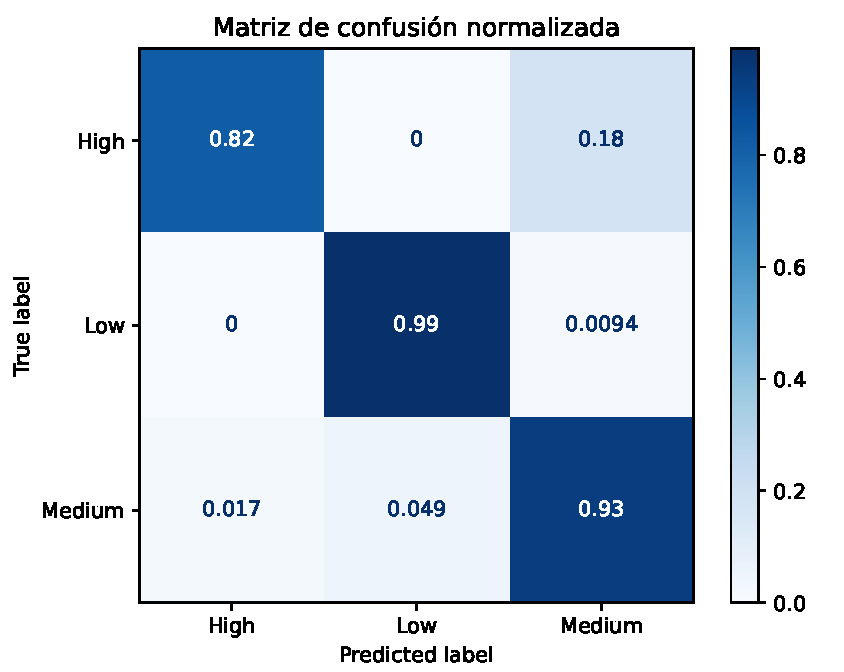
\includegraphics[width=\textwidth]{fig/08_datadriven/datadriven_05a.pdf}
        \caption{Matriz de confusión normalizada.}
        \label{fig:confusion_matrix}
    \end{subfigure}
    \hfill
    \begin{subfigure}[t]{0.43\textwidth}
        \centering
        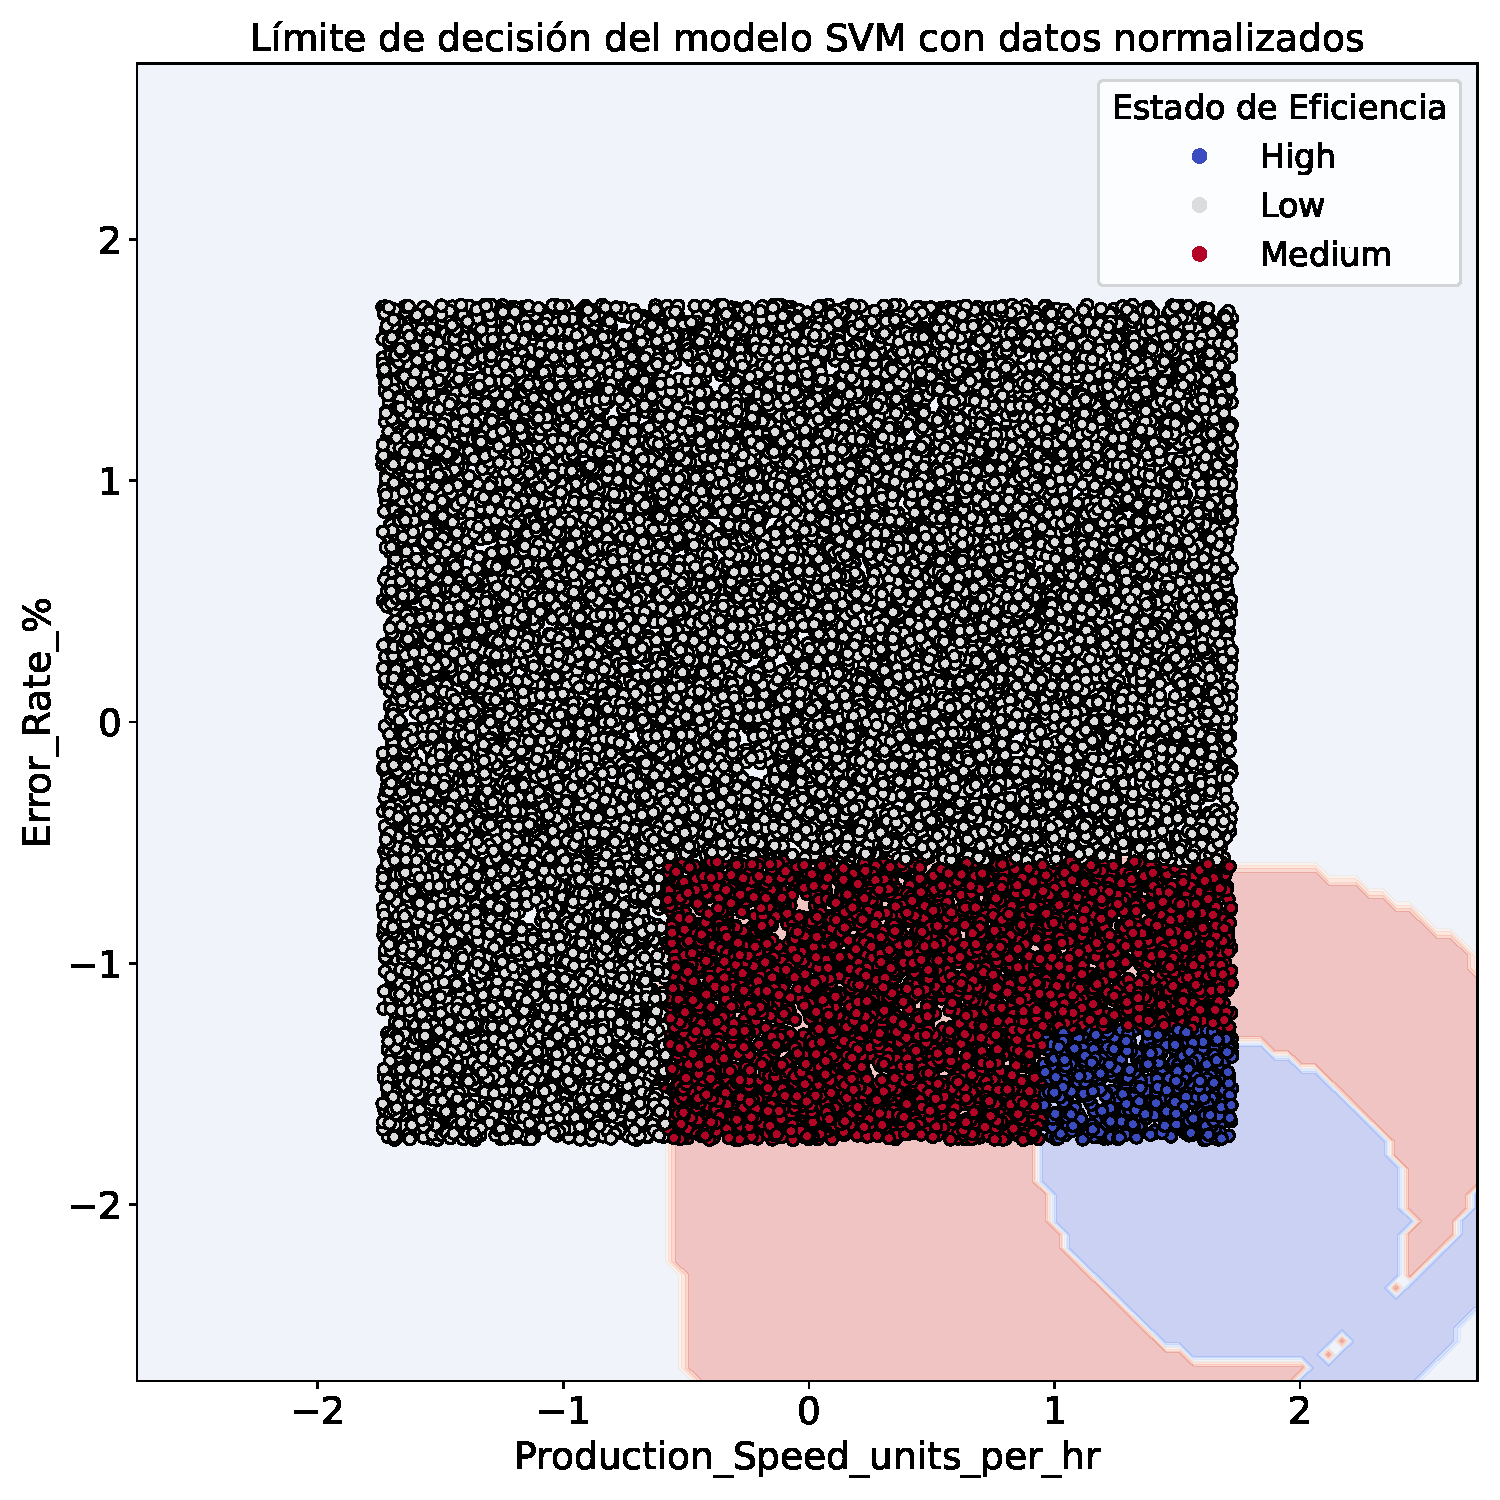
\includegraphics[width=\textwidth]{fig/08_datadriven/datadriven_05b.pdf}
        \caption{Límite de decisión del modelo SVM.}
        \label{fig:decision_boundary}
    \end{subfigure}
    \caption{Visualización del rendimiento del modelo: matriz de confusión y frontera de decisión.}
    \label{fig:model_results}
\end{figure}


\subsection{Implementación de bloques funcionales básicos}
\label{subsec:blocks}   

Esta sección describe la implementación de todos los bloques funcionales que conforman la arquitectura. La explicación comienza en el nivel más bajo con los componentes de la planta de producción (denominado como \textit{Factory Floor}), continúa con los módulos funcionales desplegados en la capa del \textit{edge}, en particular, el bloque de control y la base de datos, y se concluye con los componentes alojados en la plataforma en la nube, incluyendo el sistema de monitorización y el módulo \gls{faas} encargado de ejecutar el servicio de inferencia.


\subsubsection{Bloque de \textit{Factory Floor}}
\label{subsubsec:factoryfloor}

La planta de producción constituye la capa fundamental de la arquitectura, englobando los dispositivos \gls{iiot} y la infraestructura inalámbrica que generan y transmiten datos. Su implementación está concebida para ser adaptable a los requisitos específicos del caso de uso industrial final. No obstante, debido a la falta de acceso a un entorno real de factoría, todo el sistema se emula mediante Mininet-WiFi~\cite{mininet-wifi}. Esta herramienta permite la emulación de redes inalámbricas definidas por software, ofreciendo soporte para la configuración de nodos con recursos limitados y enlaces con capacidad variable, lo que posibilita la creación de un banco de pruebas \gls{iiot} altamente realista.  En este escenario, se implementa una topología inalámbrica de referencia compuesta por tres puntos de acceso (del inglés, \gls{ap}) programables y compatibles con OpenFlow, cada uno conectado a un número configurable de estaciones inalámbricas. Los puntos de acceso se enlazan con el módulo de control, que gestiona dinámicamente el tráfico mediante la emisión de reglas de flujo que determinan el encaminamiento de los paquetes, mientras que las estaciones inalámbricas actúan como sensores \gls{iiot} individuales.


\begin{figure}[ht!]
    \centering
    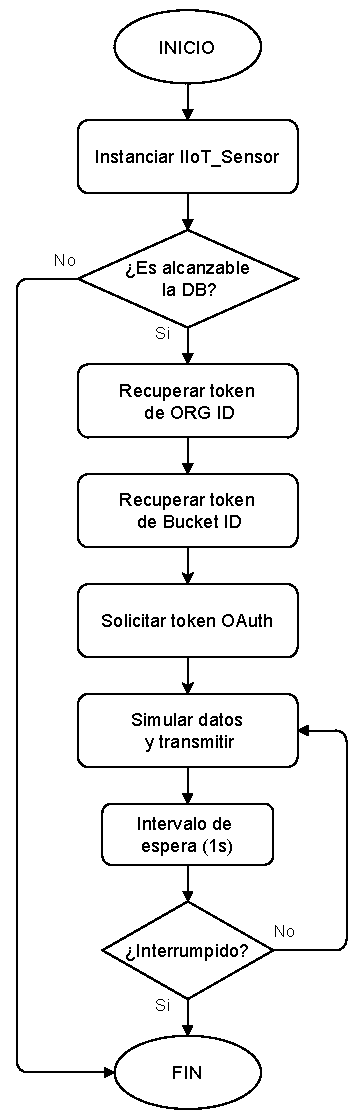
\includegraphics[width=0.33\textwidth]{fig/08_datadriven/datadriven_06.drawio.pdf}
    \caption{Diagrama de flujo que representa el ciclo de vida de la instancia \texttt{IIoT\_Sensor}, incluyendo la inicialización, los procedimientos de autenticación y la transmisión periódica de datos al módulo Base de datos.}
    \label{fig:iiot_sensor_flow}
\end{figure}

Cada sensor \gls{iiot} ejecuta una aplicación aislada basada en Python dentro de su propio espacio de nombres de red (\textit{Network Namespace}). Esta aplicación desempeña dos funciones principales: autenticar con el servicio de base de datos en el \textit{edge}, y simular y transmitir datos sintéticos de los sensores en función del análisis estadístico previamente presentado en la Sección~\ref{subsec:data}.\\
\\
La Figura~\ref{fig:iiot_sensor_flow} muestra el diagrama de flujo que describe el comportamiento emulado de los sensores \gls{iiot}. El proceso se inicia con la inicialización de los simuladores correspondientes a cada característica, basados en los parámetros estadísticos extraídos anteriormente. Tras esta fase, el sistema verifica la conectividad con el servicio de base de datos desplegado en el \textit{edge}. Una vez establecida la conexión, el sensor obtiene los identificadores de organización y planta (asignados a \textit{buckets} de datos específicos) mediante un intercambio de autenticación basado en OAuth2 con el agente de base de datos en el \textit{edge}. Con la autorización concedida, el sensor recibe un token de escritura de fina granularidad que habilita la inserción de datos únicamente en los \textit{buckets} autorizados. Posteriormente, el sensor entra en un bucle en el que simula y transmite valores de datos a intervalos de tiempo fijos (1 segundo, configurable) hasta que el proceso es interrumpido.


\subsubsection{Bloque de Control}

El módulo de control es responsable de gestionar el plano de control de las redes de los puntos de acceso (\gls{ap}) en la planta \gls{iiot}, así como de recuperar datos de los sensores \gls{iiot} a través del módulo de base de datos en la capa del \textit{edge}. Además, establece canalizaciones de inferencia con el módulo \gls{faas} desplegado en la nube, con el fin de determinar si algún sensor presenta un comportamiento anómalo. Cuando se identifican dichas anomalías, el módulo de control activa acciones de reconfiguración en el \gls{ap} correspondiente para optimizar el rendimiento de la red.\\
\\
La implementación utiliza Ryu~\cite{tomonori2013introduction} como controlador principal por dos razones fundamentales: (1) proporciona una \gls{api} sur (Sección~\ref{subsec:arquitectura_sdn}) compatible con el protocolo OpenFlow, lo que permite una configuración dinámica del plano de control de los \glspl{ap}; (2) su diseño orientado a aplicaciones facilita la creación de nuevos perfiles de control que encapsulan la lógica de decisión, incluyendo interacciones con el módulo de base de datos, solicitudes de inferencia remota al servicio en la nube y reconfiguración dinámica de la red \gls{iiot}. La lógica implementada en Ryu se detalla en el Algoritmo~\ref{alg:ryu}.\\
\\
La lógica de control se fundamenta en un bucle de decisión estrechamente integrado que combina monitorización en tiempo real, inferencia basada en \gls{ml} y aplicación de políticas de control. Cuando un \gls{ap} reenvía un paquete al controlador (mediante un evento \texttt{PacketIn}), el controlador consulta a la base de datos las lecturas recientes asociadas al sensor correspondiente. En la implementación actual, los datos recuperados son promedios agregados en una ventana temporal de 10 minutos, aunque este valor es configurable. Dichos datos se envían como petición en formato JSON a la API del módulo \gls{faas}, lo que desencadena un proceso de inferencia remota mediante el modelo de clasificación descrito previamente. El servicio \gls{faas} devuelve una etiqueta que indica si el sensor debe considerarse eficiente, ineficiente o en transición. El resultado se registra en un diccionario interno de sensores, que permite llevar un seguimiento del estado operativo de cada sensor y apoyar la toma de decisiones centralizada. Si un sensor es clasificado como ineficiente, el controlador inicia una acción de reconfiguración. En el prototipo actual, esto implica des-asociar el sensor de su \gls{ap} actual, permitiendo que se reconecte a otro punto de acceso con un rendimiento potencialmente superior. Este comportamiento demuestra la viabilidad de una reconfiguración dinámica de la red basada en \gls{ml}, que puede ser extendida o personalizada para distintos casos de uso en entornos \gls{iiot}.

\begin{algorithm}[ht!]
\DontPrintSemicolon
\KwIn{Eventos OpenFlow, paquetes IIoT}
\KwOut{Control dinámico de flujos y detección de anomalías}

Inicializar servicios de Base de Datos e Inferencia\;
Inicializar tabla MAC y lista de sensores\;

\textbf{Al conectar un AP:} establecer regla \texttt{table-miss} para enviar paquetes al controlador\;

\textbf{Al recibir un evento \texttt{packet-in}:} \\
\Indp
  Extraer datapath, puerto de entrada e información del paquete\;
  Aprender direcciones MAC origen y destino\;
  Actualizar el mapeo MAC–puerto\;
  Registrar sensores si aplica\;

  \eIf{el paquete es ARP}{
    Establecer puerto de salida en FLOOD\;
  }{
    Determinar puerto de salida a partir de la tabla MAC\;
  }

  \If{el paquete es IPv4 y corresponde a un sensor}{
    \If{el sensor está asociado a un AP y no marcado como caído}{
      Consultar métricas al módulo de BD\;
      Realizar inferencia mediante la API FaaS\;
      \If{se detecta anomalía}{
        Marcar sensor como caído\;
        Descartar paquete\;
      }
    }
    \ElseIf{el sensor estaba previamente marcado como caído pero ahora es normal}{
      Desmarcar sensor\;
    }
  }

  Instalar regla de flujo si el destino es conocido\;
  Reenviar paquete según corresponda\;
\Indm

\caption{Pseudocódigo de alto nivel del controlador Ryu.}
\label{alg:ryu}
\end{algorithm}


\subsubsection{Bloque de Base de datos}

InfluxDB~\cite{influxdb} ha sido seleccionada para la implementación del módulo de base de datos, al tratarse de una base de datos orientada a series temporales específicamente optimizada para la ingesta y consulta de datos en tiempo real. Esta elección se fundamenta en varios factores críticos para los sistemas de monitorización \gls{iiot}: su alta eficiencia en el manejo de operaciones intensivas de escritura, su soporte nativo para agregaciones en ventanas temporales y su integración inmediata con plataformas como Grafana. En particular, InfluxDB permite el almacenamiento de lecturas periódicas de sensores con marcas temporales precisas y soporta consultas agregadas con una latencia mínima. La Figura~\ref{fig:timeseries_influxdb} presenta la interfaz de usuario de InfluxDB, mostrando un ejemplo de los datos de series temporales almacenados en la base de datos. Dichos datos reflejan la evolución temporal de diferentes variables registradas por los sensores \gls{iiot}.

\begin{figure}[ht!]
    \centering
    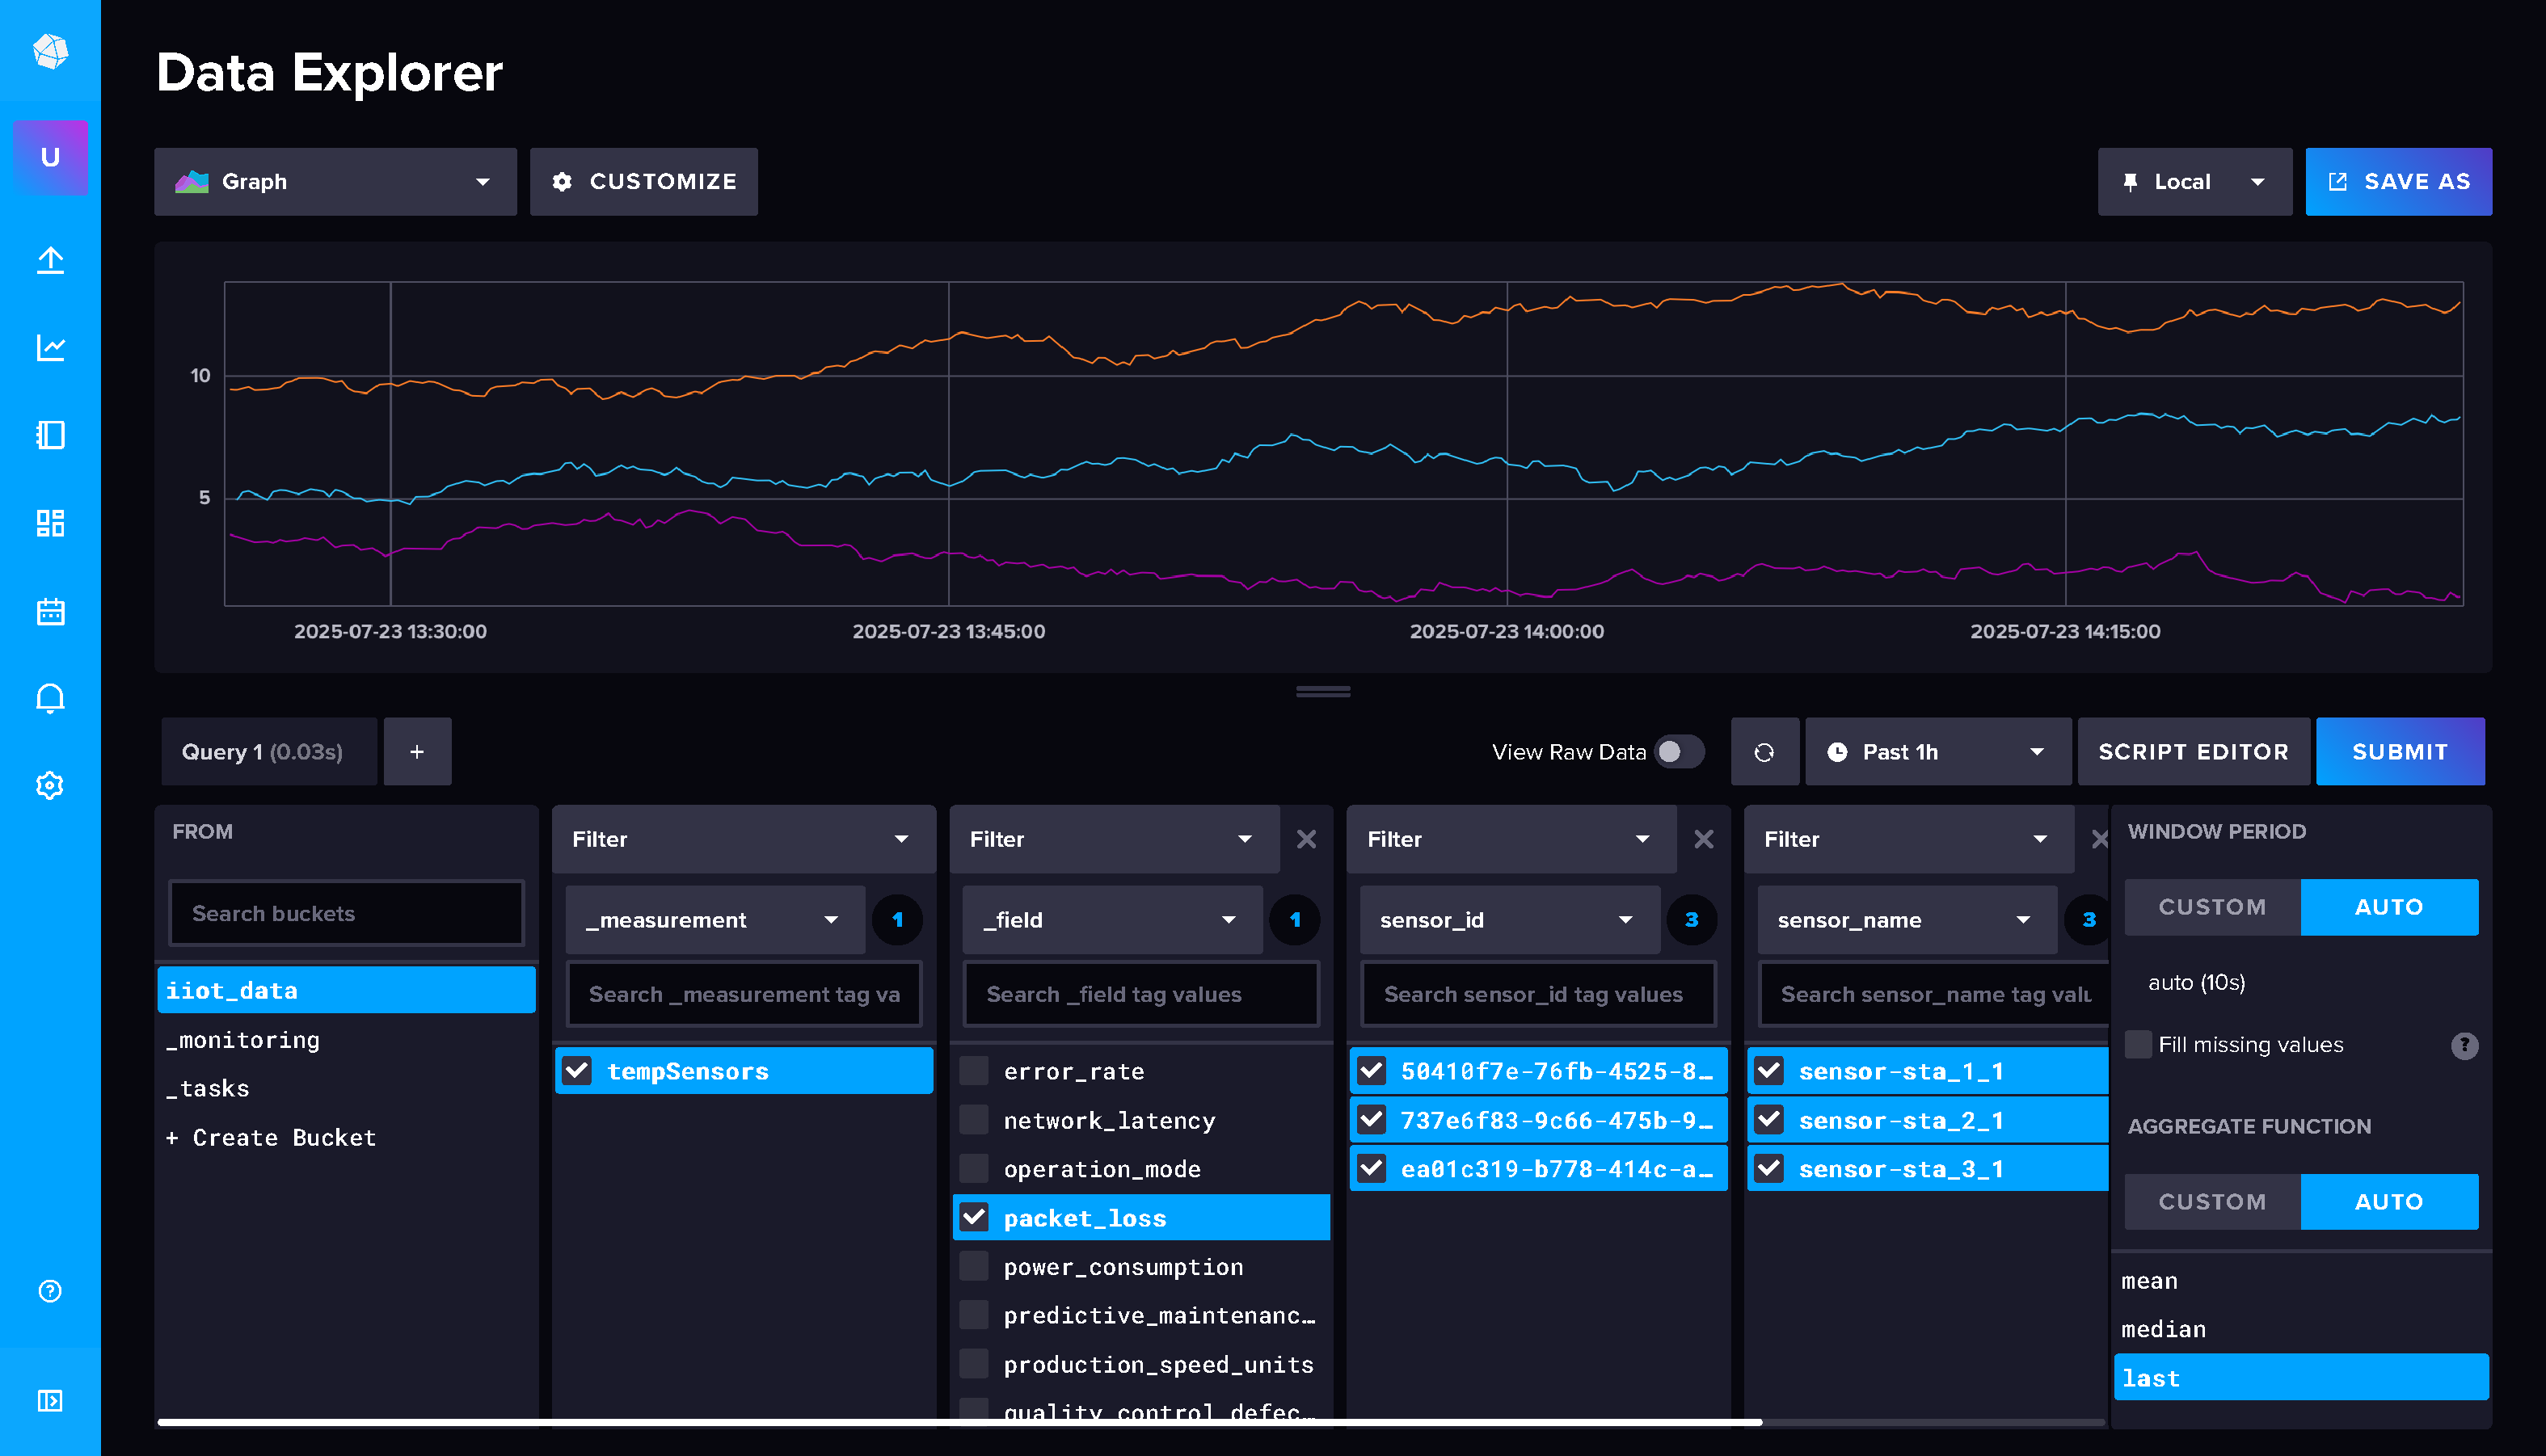
\includegraphics[width=\textwidth]{fig/08_datadriven/datadriven_07.pdf}
    \caption{Frontend de InfluxDB configurado con las series temporales de los sensores IIoT de una organización.}
    \label{fig:timeseries_influxdb}
\end{figure}


\subsubsection{Bloque de Inferencias}

En la capa de la nube, el módulo \gls{faas} aloja el servicio de inferencias que permite al módulo de control desencadenar reconfiguraciones de la red \gls{iiot}. Aunque el diseño sigue una filosofía inspirada en \gls{faas}, es decir, desplegar servicios de inferencia sin estado y bajo demanda, no se utiliza una plataforma serverless dedicada como AWS Lambda u OpenFaaS. En su lugar, el servicio se despliega como un microservicio contenedorizado gestionado mediante Kubernetes. Para ello se emplea BentoML~\cite{bentoml}, que permite empaquetar el modelo de \gls{ml} desarrollado en la Sección~\ref{subsubsec:model} y exponerlo a través de una \gls{api} RESTful. La elección de BentoML se debe a sus funcionalidades avanzadas de serialización, versionado y despliegue de modelos, así como a su soporte nativo para entornos de inferencia escalables. Este enfoque garantiza una actualización transparente de modelos y una alta disponibilidad de los puntos de inferencia bajo cargas variables, manteniendo al mismo tiempo una baja latencia.



\subsubsection{Bloque de Monitorización}

El último bloque funcional de la arquitectura corresponde al módulo de monitorización. Para este propósito se ha seleccionado Grafana~\cite{grafana}, debido a su integración directa con InfluxDB y a sus amplias capacidades de visualización. Gracias a las funcionalidades de los Dashboards y al ecosistema de complementos de Grafana, los operadores pueden construir paneles interactivos en tiempo real que muestran métricas clave de \gls{iiot}, tales como lecturas de sensores, latencia de red y estado del sistema, obtenidas directamente de InfluxDB. La Figura~\ref{fig:grafana} ilustra la interfaz de usuario configurada, la cual proporciona a los operadores de planta una visión integral y en tiempo real de la topología completa de la red \gls{iiot} y de su rendimiento operativo. 


\begin{figure}[ht!]
    \centering
    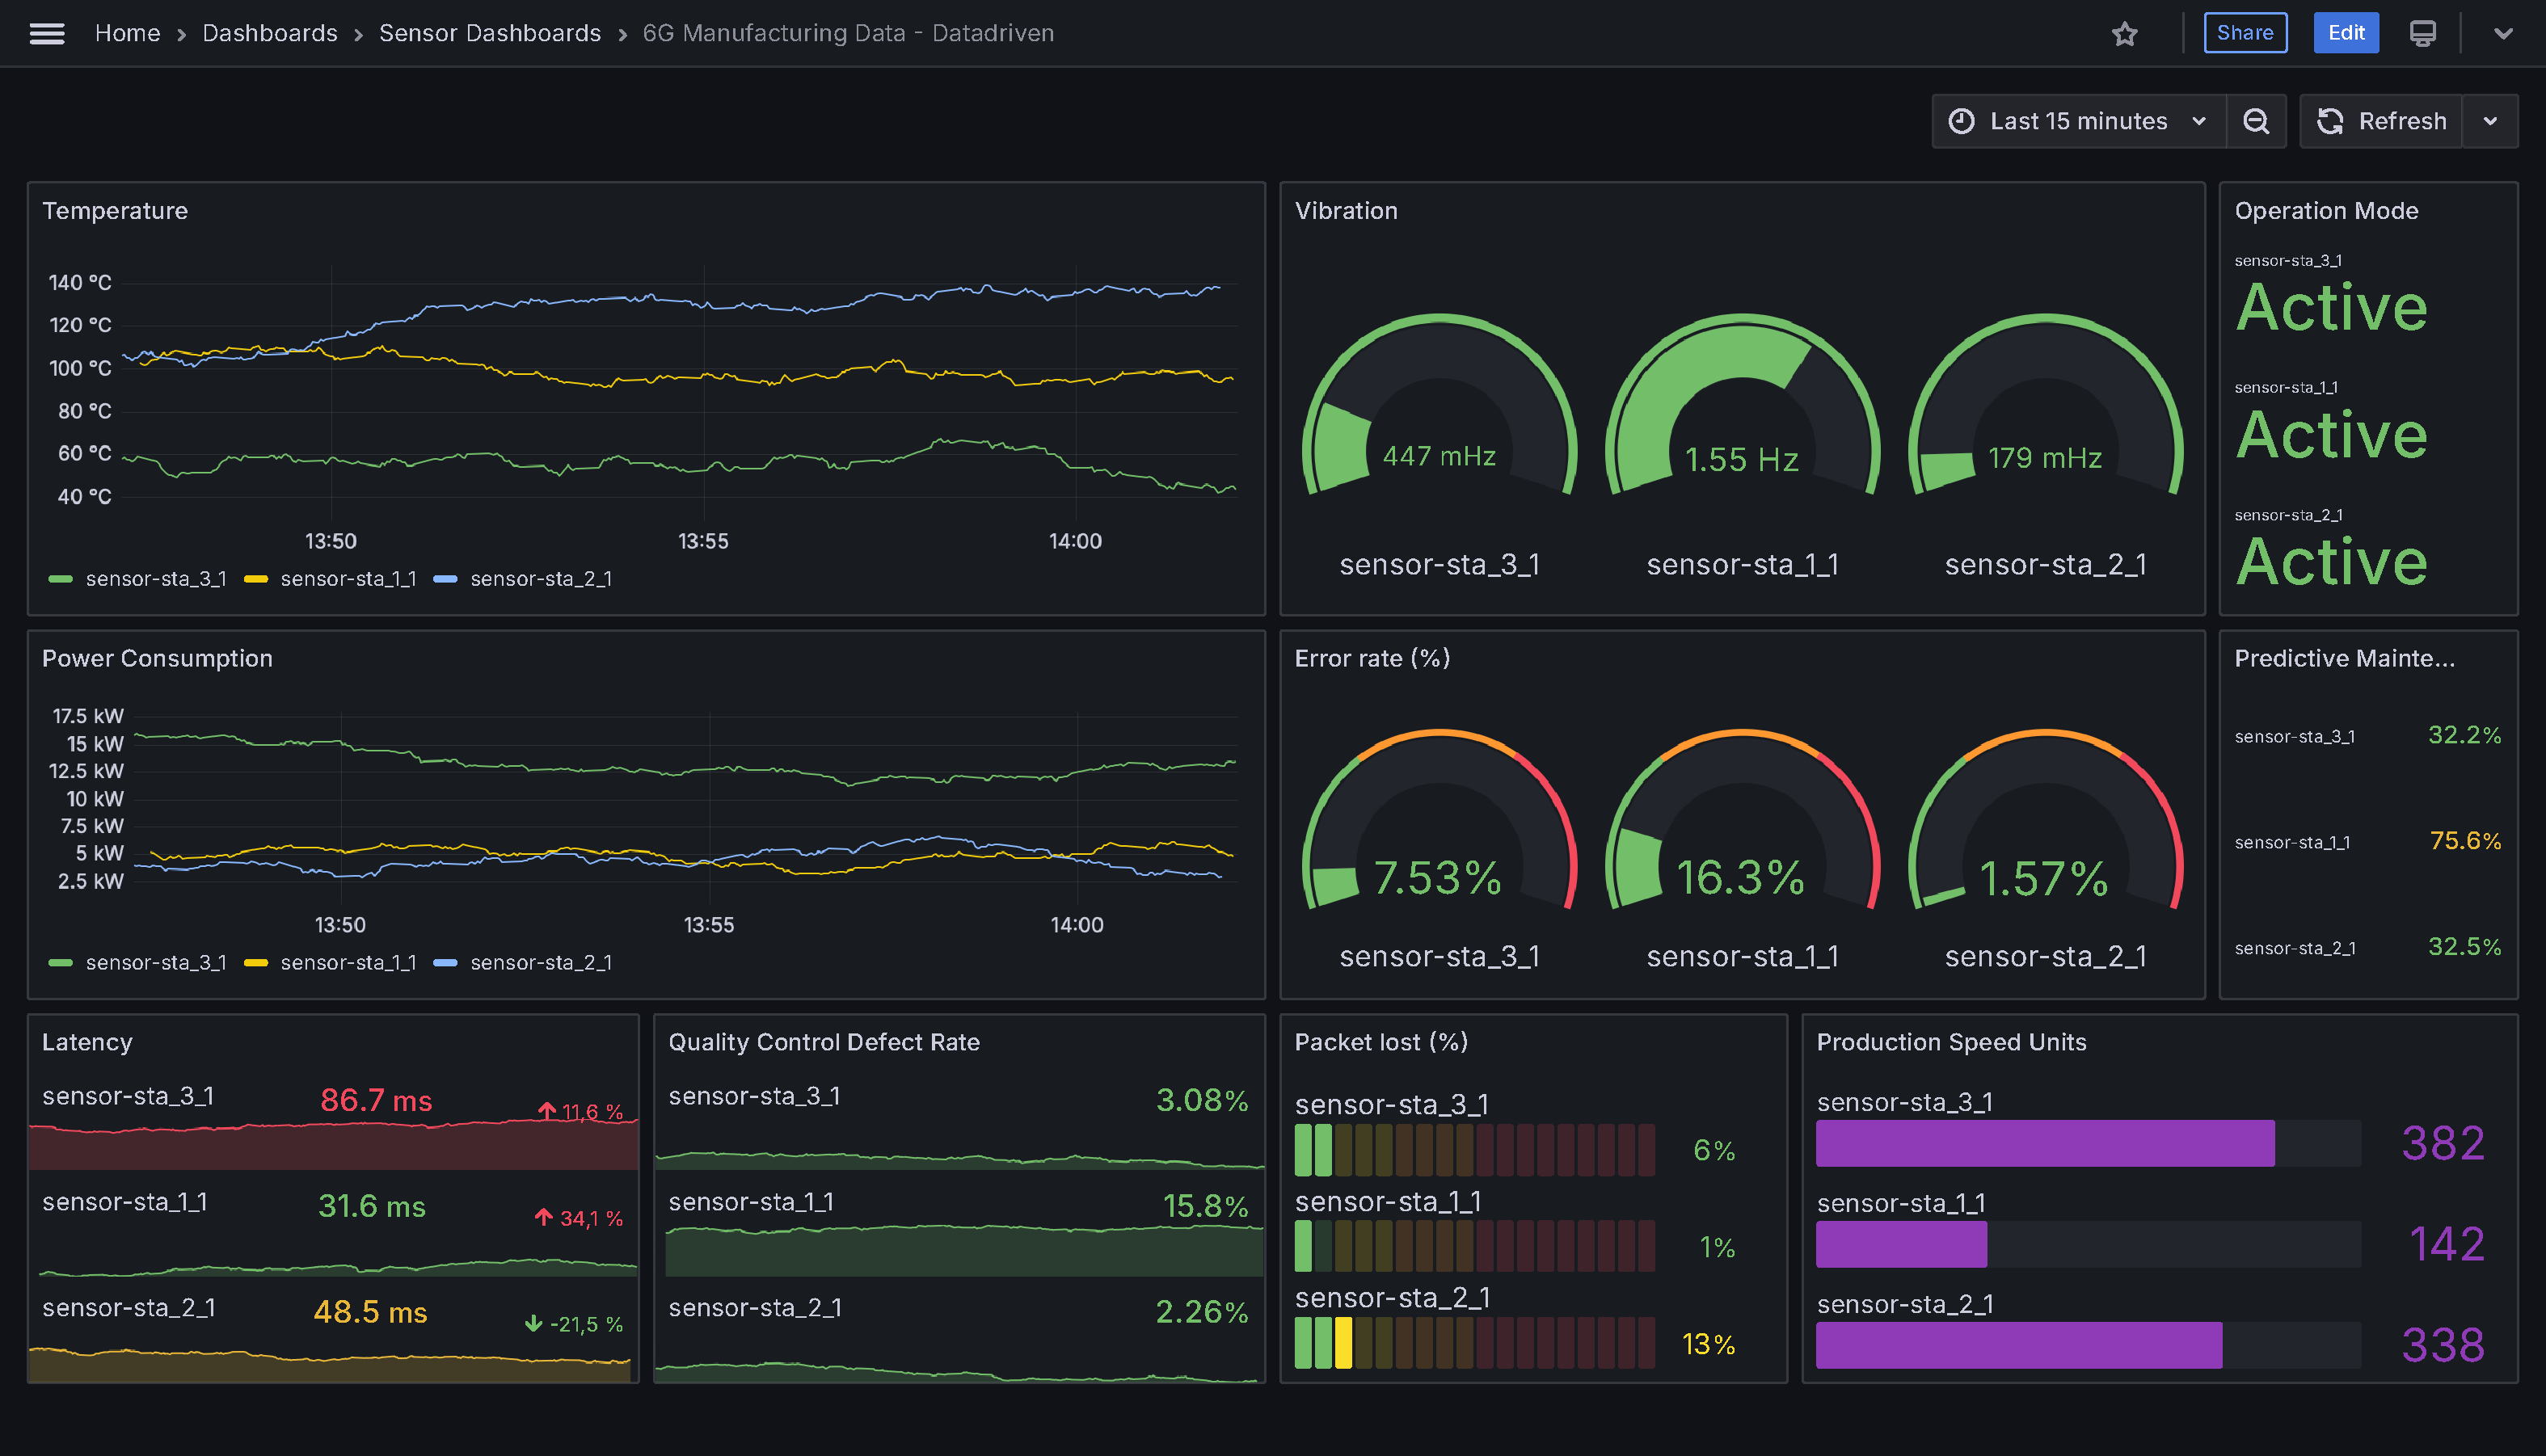
\includegraphics[width=\textwidth]{fig/08_datadriven/datadriven_08.pdf}
    \caption{Panel de control del frontend de Grafana configurado con toda la información de los sensores IIoT.}
    \label{fig:grafana}
\end{figure}


\subsection{Despliegue de arquitectura en Kubernetes}
\label{subsec:k8s}

Esta sección describe la arquitectura completa de despliegue utilizada para integrar todos los componentes del sistema \gls{iiot} propuesto, siguiendo un enfoque de microservicios basado en Kubernetes. La contenerización constituye la estrategia de despliegue preferida para sistemas complejos compuestos por múltiples servicios ligeros e independientes que deben interactuar para proporcionar una funcionalidad cohesiva. Al aislar cada bloque lógico como un contenedor autónomo, el sistema se vuelve más modular, portable y sencillo de escalar o actualizar de manera independiente. Kubernetes amplía este modelo mediante características nativas como autoescalado, balanceo de carga, tolerancia a fallos, almacenamiento persistente a través de \gls{pvc} y comunicación transparente entre servicios. Si bien herramientas más simples como Docker Compose permiten orquestar despliegues básicos, los entornos de producción suelen requerir plataformas más avanzadas como Kubernetes, OpenShift, Nomad o Rancher. Estos orquestadores ofrecen funcionalidades críticas a nivel empresarial, tales como comprobaciones de estado, alta disponibilidad, descubrimiento de servicios y despliegue declarativo. La motivación para adoptar este modelo con Kubernetes radica en su capacidad para proporcionar modularización, escalabilidad, tolerancia a fallos y una gestión detallada de servicios, aspectos difíciles de lograr en despliegues sobre hardware dedicado o con orquestadores más simples.\\
\\
Para soportar el despliegue, se configuró un clúster de Kubernetes de tres nodos (utilizando \texttt{containerd} como motor de contenedores) mediante la herramienta oficial \texttt{kubeadm}, que ofrece un método simplificado para inicializar y gestionar despliegues de Kubernetes. Como se muestra en la parte izquierda de la Figura~\ref{fig:cluster-scheme}, el clúster está compuesto por: (1) un nodo maestro que ejecuta el plano de control de Kubernetes. Este nodo es responsable de gestionar el estado del clúster, incluyendo la planificación de cargas de trabajo, la distribución de configuraciones y la exposición de \glspl{api} para la administración de servicios. El nodo maestro no ejecuta servicios de aplicación, sino que orquesta los despliegues en todo el clúster. (2) Dos nodos de trabajo, que alojan los componentes reales de la aplicación. Estos nodos ejecutan los servicios contenerizados. Kubernetes organiza los contenedores en unidades lógicas denominadas pods, que representan la unidad mínima desplegable. Cada pod suele ejecutar uno o varios contenedores estrechamente acoplados que comparten recursos de red y almacenamiento. En nuestro despliegue, cada componente central (p. ej., base de datos, controlador, \gls{faas}) se ejecuta en su propio pod, gestionado por el planificador de Kubernetes. Para garantizar la conectividad entre pods de distintos nodos, se emplea Calico como complemento \gls{cni}. Calico proporciona una red superpuesta segura y un mecanismo de aplicación de políticas para la comunicación entre pods, tanto dentro de un mismo nodo como entre nodos distintos.

\begin{figure}[ht!]
    \centering
    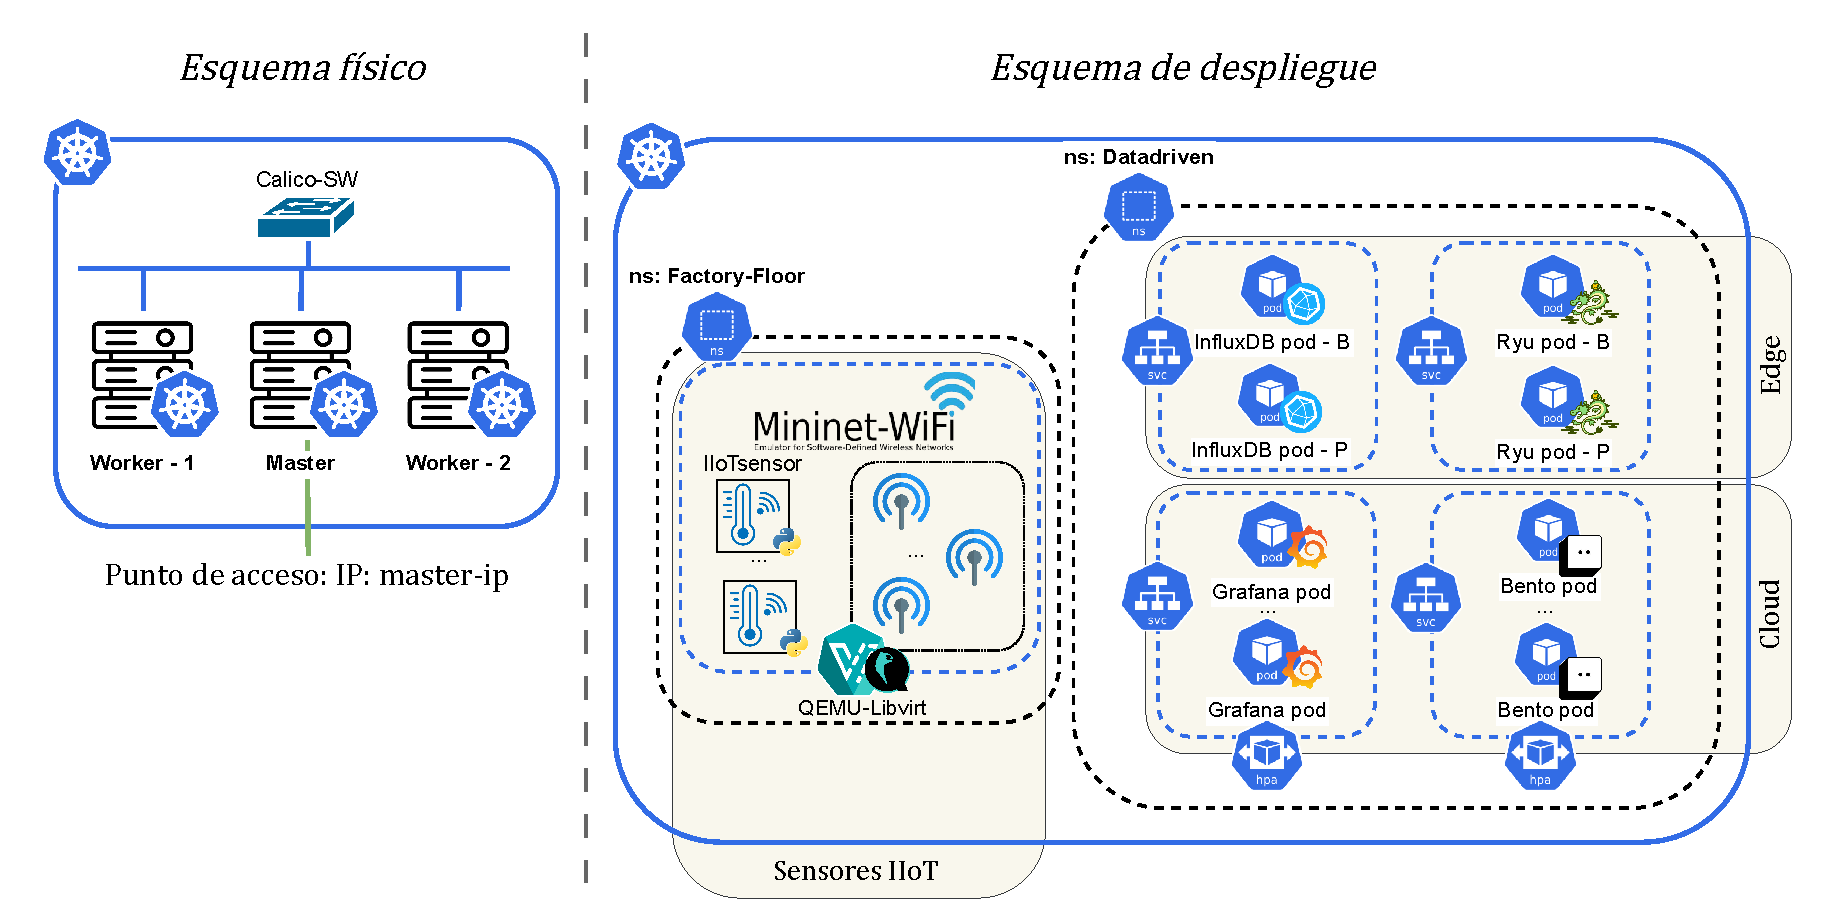
\includegraphics[width=0.95\textwidth]{fig/08_datadriven/datadriven_09.drawio.pdf}
    \caption{Descripción física y lógica del despliegue del clúster.}
    \label{fig:cluster-scheme}
\end{figure}

El esquema lógico de despliegue se muestra en la parte derecha de la Figura~\ref{fig:cluster-scheme}. En él se ilustra cómo la infraestructura física (nodos del clúster) se mapea hacia los entornos virtuales (namespaces), servicios y pods. La arquitectura se encuentra lógicamente dividida en dos namespaces (\texttt{ns}): \texttt{Factory-floor} y \texttt{Datadriven}. El namespace \texttt{Factory-floor} emula el entorno \gls{iiot} mediante una máquina virtual desplegada a través de KubeVirt y QEMU-Libvirt. Esta máquina virtual ejecuta Mininet-WiFi, dentro del cual se instancian topologías de red inalámbricas y se simulan sensores \gls{iiot}. Estos sensores se comportan de acuerdo con lo descrito en la Sección~\ref{subsubsec:factoryfloor}. \\
\\
Por su parte, \texttt{Datadriven} aloja todos los servicios del \textit{edge} y \textit{cloud} necesarios para la toma de decisiones y la monitorización. Entre estos se incluyen los servicios de borde, el controlador Ryu y la base de datos InfluxDB, desplegados en configuración activo-respaldo para proporcionar resiliencia, así como el servicio de inferencia BentoML y los paneles de Grafana, ambos configurados con \gls{hpa}, lo que permite escalar dinámicamente en función del uso de CPU y memoria para mantener el rendimiento bajo cargas variables. Un resumen de los recursos hardware asignados para ejecutar la infraestructura se recoge en la Tabla~\ref{tab:hardware-specs}.

\begin{table}[ht!]
\centering
\begin{tabular}{|p{6cm}|p{7cm}|}
\hline
\textbf{Componente} & \textbf{Especificaciones}\\
\hline
Nodos del clúster de Kubernetes & 16 GB RAM; 8 vCPUs; formato Blade\\
\hline
Máquina virtual con Mininet-WiFi & 4 GB RAM; 4 vCPUs\\
\hline
\end{tabular}
\caption{Especificaciones de los recursos hardware asignados al despliegue.}
\label{tab:hardware-specs}
\end{table}

\subsubsection{Mecanismos de escalabilidad y tolerancia a fallos}

Para habilitar un escalado adaptativo bajo cargas de trabajo variables, se configuran \glspl{hpa} para los servicios de Grafana y BentoML. Cada \gls{hpa} mantiene un mínimo de una y un máximo de cinco réplicas de pod. El escalado se activa automáticamente cuando la utilización de CPU supera el 70\%, garantizando que los servicios permanezcan receptivos durante los picos de carga. Los límites de recursos de CPU se definen con un mínimo de 100 millicores y un máximo de 500 millicores por pod.\\
\\
Para los componentes con estado, como InfluxDB y Ryu, no se emplea \gls{hpa}. En su lugar, estos servicios se despliegan con redundancia activa-en-espera (del inglés, \textit{active-standby}) para proporcionar tolerancia a fallos y asegurar la continuidad del servicio. Se aprovisionan dos pods para cada componente: uno actúa como nodo primario, gestionando tanto las operaciones de lectura como de escritura, mientras que el segundo permanece en modo de espera. Las solicitudes de escritura se replican en ambas instancias para mantener la consistencia. En caso de fallo del nodo primario, la instancia en espera se promueve automáticamente a activa, asumiendo la totalidad de las responsabilidades operativas con una mínima interrupción del sistema. El servicio nativo de Kubernetes gestiona el balanceo de carga entre réplicas, enrutando automáticamente el tráfico hacia todos los pods activos. Los pods creados recientemente son etiquetados e integrados en la malla de servicios sin necesidad de reconfiguración. Este enfoque híbrido, que combina escalado automático para servicios sin estado y redundancia manual para aquellos con estado, garantiza tanto la elasticidad del rendimiento como la alta disponibilidad a lo largo de la arquitectura desplegada.


\subsubsection{Flujo de datos entre componentes de la arquitectura}

Tras la descripción del clúster de Kubernetes y del despliegue lógico, se examina ahora el flujo operativo de datos entre los principales componentes del sistema, ilustrado en la Figura~\ref{fig:dataflow}.

\begin{figure}[ht!]
    \centering
    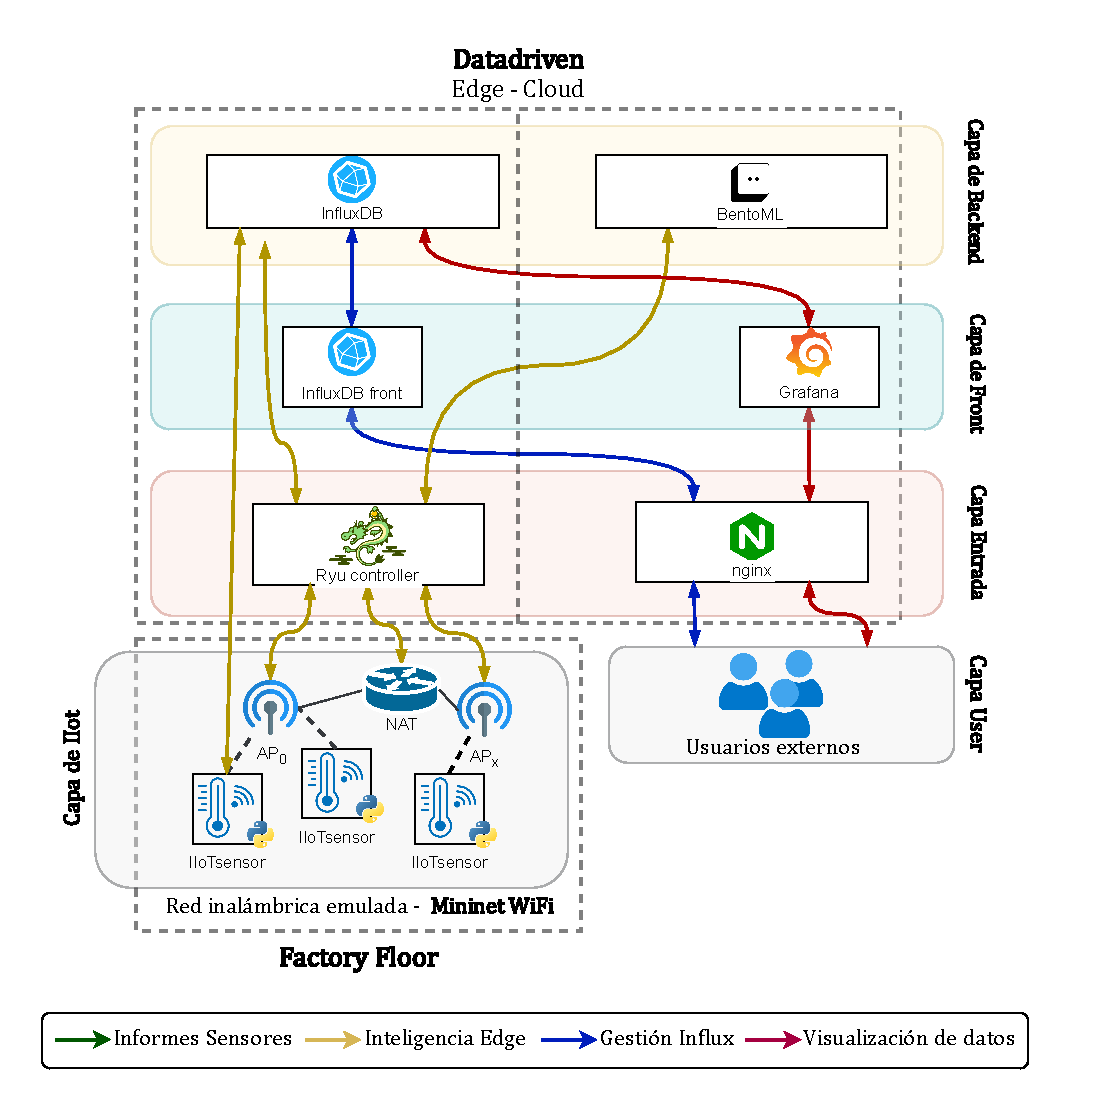
\includegraphics[width=0.8\textwidth]{fig/08_datadriven/datadriven_10.drawio.pdf}
    \caption{Flujos de datos entre componentes de la arquitectura.}
    \label{fig:dataflow}
\end{figure}

En la parte inferior izquierda del diagrama, la capa \gls{iiot} representa el entorno de fábrica emulado mediante Mininet-WiFi, que instancia una red mallada inalámbrica habilitada con \gls{sdn}, compuesta por nodos sensores virtuales \gls{iiot} (denotados como \texttt{IIoTSensor}) y \gls{ap}. Cada sensor genera y transmite mediciones periódicas, tal y como se indicó en la Sección~\ref{subsubsec:factoryfloor}. Los paquetes generados atraviesan la red \gls{sdn}, alcanzan un punto de acceso (AP) y son enrutados a través de un gateway NAT hacia el controlador Ryu en la capa de entrada. El controlador Ryu procesa los mensajes procedentes de la capa \gls{iiot} y habilita la evaluación de la eficiencia de los sensores, así como la monitorización de la red en tiempo real, consultando dinámicamente dos servicios: (1) InfluxDB, para recuperar métricas recientes de los sensores, y (2) BentoML, para invocar la canalización de inferencia que determina si un sensor se encuentra en un estado anómalo. En función de los resultados de estas interacciones, el controlador puede activar acciones de reconfiguración, como disociar un sensor de su AP actual y redirigirlo hacia otro con mejor rendimiento.\\
\\
De manera paralela, los usuarios externos interactúan con el sistema a través de la capa \textit{Users}. Todas las solicitudes HTTP entrantes son encaminadas mediante un proxy Nginx, que actúa como único punto de acceso externo al sistema. Desde allí, el proxy reenvía el tráfico hacia dos servicios de \textit{front-end}: (1) Grafana, que consulta periódicamente InfluxDB para generar los paneles en tiempo real con los datos de los sensores; y (2) la interfaz web de InfluxDB, que permite a los administradores del sistema inspeccionar, consultar y gestionar directamente las series temporales de datos.\\
\\
Este diseño de flujo de datos multinivel permite la monitorización continua, la inferencia inteligente y la observabilidad por parte de los usuarios, manteniendo al mismo tiempo la separación arquitectónica entre dispositivos emulados, lógica de control y servicios orientados al usuario.


\section{Evaluación experimental}
\label{sec:eva}

En esta sección se presenta la evaluación experimental de la arquitectura propuesta, organizada en tres subsecciones: (i) \emph{Utilización de recursos y escalabilidad}, donde se analizan las métricas de CPU, memoria y tiempo de despliegue en función de la carga del sistema y del número de sensores \gls{iiot}; (ii) \emph{Latencia de inferencia e ingestión de datos}, que mide el tiempo promedio de inferencia y la latencia de ingestión de datos en el módulo de base de datos utilizando la herramienta \texttt{hey}; y (iii) \emph{Tiempo promedio de reconfiguración de red}, en el que se estudia el retardo medio de reconfiguración de la red a medida que varía el número de sensores \gls{iiot}. Todas las pruebas se llevaron a cabo en un servidor DELL PowerEdge R650 equipado con dos procesadores Intel Xeon Silver-4310 a 2.10~GHz (18 MB de caché) y 512 GB de memoria RAM DDR4. El objetivo de esta evaluación experimental es cuantificar el rendimiento de la arquitectura y evaluar su flexibilidad y escalabilidad, así como su capacidad de adaptarse a diferentes requisitos de \gls{qos} y de reconfigurarse de manera autónoma en respuesta a condiciones operativas cambiantes.     

\subsection{Utilización de recursos y escalabilidad}

En esta subsección se evalúa el rendimiento y la escalabilidad de la arquitectura propuesta, centrándose exclusivamente en los componentes de \textit{Edge} y \textit{Cloud}. La capa de \textit{Factory floor} depende en gran medida de los requisitos específicos de cada caso de uso y puede variar sustancialmente en función del entorno operativo. Tal y como se explicó en secciones anteriores, en nuestra implementación, la capa de \textit{Factory floor} se emula mediante una máquina virtual que ejecuta Mininet-WiFi, reproduciendo una topología inalámbrica \gls{sdn} con nodos \gls{iiot} con recursos limitados. Sin embargo, para los fines de este análisis, restringimos el alcance de la evaluación a los bloques funcionales principales ubicados en los niveles de \textit{Edge} y \textit{Cloud} de la arquitectura. Comenzamos analizando el tiempo de despliegue de todo el sistema, desglosado en sus distintas fases. La Tabla~\ref{tab:deployment-times} presenta el tiempo medio de ejecución de cada etapa, junto con su intervalo de confianza (IC), repitiendo el despliegue completo 20 veces. El tiempo medio total de despliegue asciende aproximadamente a $269.15 \pm 1.69$ segundos.

\begin{table}[ht!]
\centering
\begin{tabular}{|l|c|}
\hline
\textbf{Etapa} & \textbf{Tiempo (s)} \\
\hline
Dashboard & $2.85 \pm 0.17$ \\ \hline
Destrucción de despliegues & $4.70 \pm 0.22$ \\ \hline
Proveedor de máquinas virtuales & $10.10 \pm 0.34$ \\ \hline
Configuración del nodo maestro & $39.95 \pm 1.30$ \\ \hline
Configuración del servidor de métricas & $3.05 \pm 0.10$ \\ \hline
Configuración de \textit{namespaces} & $2.70 \pm 0.22$ \\ \hline
Despliegue de \texttt{datadriven} & $5.15 \pm 0.49$ \\ \hline
Instalación de \texttt{containerd} y Kubernetes & $198.65 \pm 1.36$ \\ \hline
Asociación del \textit{worker-1} & $1.00 \pm 0.00$ \\ \hline
Asociación del \textit{worker-2} & $1.00 \pm 0.00$ \\ \hline
Total & $269.15 \pm 1.69$ \\
\hline
\end{tabular}
\caption{Tiempo de despliegue (media $\pm$ IC) por cada etapa.}
\label{tab:deployment-times}
\end{table}

La fase más costosa en tiempo es la instalación del entorno de ejecución de contenedores y del clúster de Kubernetes, que incluye la configuración de \texttt{containerd} y de los componentes esenciales de Kubernetes. Este paso requiere aproximadamente $198.65 \pm 1.36$ segundos, lo que representa cerca del 74\% del tiempo total de despliegue. A continuación, la configuración del nodo \textit{maestro} requiere alrededor de $39.95 \pm 1.30$ segundos, incluyendo la inicialización del clúster y la configuración del plano de control. Las fases posteriores, como el aprovisionamiento de máquinas virtuales ($10.10 \pm 0.34$ s), la configuración de \textit{namespaces} ($2.70 \pm 0.22$ s), y el despliegue de los servicios \texttt{datadriven} ($5.15 \pm 0.49$ s), aportan una contribución marginal al tiempo total. La adición de nodos \textit{worker} es prácticamente instantánea, con solo un segundo requerido por cada uno, lo que pone de manifiesto la eficiencia del proceso de escalado horizontal una vez que el clúster está operativo. Estos resultados confirman que, a pesar de la complejidad del sistema, el proceso de despliegue es eficiente en tiempo y repetible, lo que permite un restablecimiento rápido en entornos dinámicos o multiusuario.\\
\\
Tras el análisis del tiempo de despliegue, examinamos los patrones de consumo de memoria de los bloques funcionales ubicados en los niveles de \textit{Edge} y \textit{Cloud}. La Tabla~\ref{tab:service-consumption} muestra el uso promedio de memoria, expresado en MiB, junto con los correspondientes intervalos de confianza, para cada servicio principal, BentoML, Grafana, InfluxDB y Ryu, en función del número de estaciones \gls{iiot} (STAs) por \gls{ap}. Como era de esperar, BentoML presenta el crecimiento más significativo en el consumo de memoria conforme aumenta la carga de la red. Partiendo de $204.00$~MiB con una sola STA, su uso alcanza un máximo cercano a $1005.46$~MiB para 9 STAs por AP. A partir de este punto, el consumo de memoria fluctúa moderadamente, pero se mantiene dentro de un rango operativo estable entre aproximadamente 750 y 985~MiB. Estos resultados confirman que BentoML escala con el número de peticiones de inferencia concurrentes, aunque el escalado horizontal mitiga la saturación de recursos, tal y como se describió en la configuración de autoescalado.\\
\\
Grafana mantiene un uso de memoria relativamente estable en todas las configuraciones evaluadas. Con una línea base de $91.43 \pm 0.63$~MiB, su consumo aumenta ligeramente hasta alcanzar $101.78 \pm 0.90$~MiB con 17 STAs, antes de disminuir cuando se generan menos operaciones de renderizado en escenarios de mayor carga, posiblemente debido a limitaciones de actualización o mecanismos de \textit{throttling} de visualización (Una técnica que limita la velocidad a la que se ejecuta una función de visualización durante un periodo de tiempo específico, garantizando que las operaciones se realicen a un ritmo controlado y constante, en lugar de sobrecargar el sistema). Se observa una caída brusca tras las 23 STAs, probablemente causada por optimizaciones internas del panel o efectos de saturación.\\
\\
InfluxDB muestra un incremento gradual y consistente en el uso de memoria a medida que aumenta el número de STAs. Comenzando en $88.76 \pm 0.31$~MiB con una STA, alcanza $131.57 \pm 1.14$~MiB con 29 STAs. Este comportamiento refleja la tendencia esperada en bases de datos de series temporales bajo un mayor volumen de operaciones de escritura y consulta, sin mostrar indicios de degradación de rendimiento o fugas de memoria.

\begin{table}[ht!]
\centering
\begin{tabular}{|c|c|c|c|c|}
\hline
\textbf{STAs/AP} & \textbf{BentoML} & \textbf{Grafana} & \textbf{InfluxDB} & \textbf{Ryu} \\
\hline
1  & $204.00 \pm 0.00$ & $91.43 \pm 0.63$ & $88.76 \pm 0.31$ & $56.00 \pm 0.00$ \\ \hline
3  & $371.42 \pm 12.20$ & $93.85 \pm 0.32$ & $90.19 \pm 0.49$ & $56.00 \pm 0.00$ \\ \hline
5  & $870.93 \pm 22.28$ & $95.09 \pm 0.39$ & $92.17 \pm 0.52$ & $56.00 \pm 0.00$ \\ \hline
7  & $985.79 \pm 26.21$ & $98.42 \pm 0.90$ & $96.65 \pm 0.46$ & $56.00 \pm 0.00$ \\ \hline
9  & $1005.46 \pm 19.87$ & $97.51 \pm 0.81$ & $100.49 \pm 0.48$ & $56.00 \pm 0.00$ \\ \hline
11 & $995.21 \pm 21.21$ & $96.17 \pm 0.59$ & $104.32 \pm 0.50$ & $56.00 \pm 0.00$ \\ \hline
13 & $754.61 \pm 33.64$ & $89.65 \pm 1.93$ & $106.57 \pm 0.64$ & $56.10 \pm 0.05$ \\ \hline
15 & $939.22 \pm 29.45$ & $99.89 \pm 0.60$ & $111.89 \pm 0.65$ & $56.12 \pm 0.05$ \\ \hline
17 & $883.30 \pm 27.66$ & $101.78 \pm 0.90$ & $116.83 \pm 0.64$ & $56.12 \pm 0.05$ \\ \hline
19 & $753.59 \pm 34.64$ & $101.27 \pm 0.67$ & $121.23 \pm 0.61$ & $56.10 \pm 0.04$ \\ \hline
21 & $922.75 \pm 30.98$ & $98.84 \pm 0.48$ & $123.76 \pm 0.67$ & $56.11 \pm 0.05$ \\ \hline
23 & $978.33 \pm 29.24$ & $85.62 \pm 2.12$ & $124.17 \pm 0.55$ & $56.23 \pm 0.09$ \\ \hline
25 & $985.62 \pm 29.87$ & $67.03 \pm 0.02$ & $124.97 \pm 0.94$ & $56.41 \pm 0.12$ \\ \hline
27 & $867.90 \pm 27.61$ & $67.00 \pm 0.00$ & $128.22 \pm 1.04$ & $56.21 \pm 0.08$ \\ \hline
29 & $940.72 \pm 33.25$ & $67.00 \pm 0.00$ & $131.57 \pm 1.14$ & $56.22 \pm 0.08$ \\ 
\hline
\end{tabular}
\caption{Consumo de memoria (MiB) promedio ($\pm$ IC) por servicio en función de las STAs por AP.}
\label{tab:service-consumption}
\end{table}

En contraste, Ryu demuestra un uso constante de memoria a lo largo de todas las pruebas, manteniéndose en torno a 56~MiB independientemente de la carga del sistema. Esta consistencia se debe a su naturaleza ligera como controlador \gls{sdn}, cuya lógica de control permanece independiente del número de STAs una vez que la topología ha sido instanciada. En conjunto, estos resultados confirman la eficiencia en el uso de memoria y la escalabilidad de la arquitectura. Los servicios se comportan de forma predecible bajo condiciones de estrés, y sus perfiles de recursos validan la decisión de adoptar una estrategia de despliegue basada en microservicios.\\
\\
La Tabla~\ref{tab:cpu-usage} presenta el uso promedio de CPU en milicores\footnote{Una unidad de medida de recursos de CPU que representa una milésima parte de un núcleo (1/1000), es decir, 1000 milicores equivalen a un núcleo completo.} para cada componente principal de la arquitectura, BentoML, Grafana, InfluxDB y Ryu, en función del número de nodos sensores \gls{iiot}. Como era de esperar, BentoML muestra un incremento pronunciado en el consumo de CPU a medida que aumenta el número de sensores \gls{iiot}, alcanzando su máximo en 25 STAs con aproximadamente $301.29 \pm 26.98$ milicores. Esta tendencia pone de manifiesto la demanda computacional asociada a la ejecución de tareas de inferencia \gls{ai}/\gls{ml} conforme se ingiere un mayor volumen de datos. Sin embargo, a partir de este punto la carga desciende ligeramente, probablemente debido a efectos de balanceo de carga o \textit{batching} de inferencias a nivel de servicio. InfluxDB también presenta un crecimiento sostenido en el consumo de CPU, con un incremento desde $13.89 \pm 0.36$ milicores con una STA hasta un máximo de $340.67 \pm 37.68$ milicores con 25 STAs. Este comportamiento es consistente con el esperado aumento en operaciones de escritura y volumen de consultas derivado de una mayor actividad de sensores.\\
\\
Ryu, el módulo de control, muestra un incremento significativo en el uso de CPU entre 1 y 9 STAs, alcanzando $168.85 \pm 8.74$ milicores, para después fluctuar de forma moderada. Esto indica que Ryu participa activamente en el bucle de control y en la gestión de eventos OpenFlow, en particular durante las reconfiguraciones de red y las decisiones de encaminamiento. En contraste, Grafana se mantiene relativamente ligero hasta alcanzar las 11 STAs, momento a partir del cual se observa una caída brusca en su consumo de CPU, estabilizándose en torno a $2.6$ milicores para 25 o más STAs/AP. Este comportamiento se atribuye a mecanismos internos de optimización, almacenamiento en caché y al hecho de que Grafana únicamente renderiza paneles de forma periódica, reduciendo así su carga durante periodos de operación en estado estable.\\
\\
Para profundizar en el comportamiento de escalado de BentoML, se analizó con mayor detalle el consumo de CPU en el escenario con 25 STAs por AP. Tal y como se ilustra en la Figura~\ref{fig:time_advance_consumption_stas25__ns_bentoml_datadriven}, se observa un pico inicial de uso de CPU debido a que una única instancia gestiona toda la carga entrante. No obstante, el sistema va generando progresivamente réplicas adicionales de BentoML en respuesta al aumento de demanda, distribuyendo eficazmente la carga. Este comportamiento refleja la activación del \gls{hpa} y demuestra que, aunque la arquitectura escala con el número de dispositivos \gls{iiot} activos, los componentes presentan distintos grados de sensibilidad frente al incremento de la carga. En particular, BentoML e InfluxDB resultan ser los servicios más intensivos en CPU, lo que requiere especial atención en las estrategias de dimensionamiento y autoescalado.

\begin{table}[ht!]
\centering
\begin{tabular}{|c|c|c|c|c|}
\hline
\textbf{STAs/AP} & \textbf{BentoML} & \textbf{Grafana} & \textbf{InfluxDB} & \textbf{Ryu} \\
\hline
1  & $8.43 \pm 0.53$   & $11.78 \pm 0.27$ & $13.89 \pm 0.36$ & $6.57 \pm 0.60$ \\ \hline
3  & $59.31 \pm 7.20$  & $25.45 \pm 1.43$ & $46.25 \pm 2.31$ & $41.65 \pm 3.98$ \\ \hline
5  & $178.19 \pm 12.43$& $40.61 \pm 1.50$ & $89.91 \pm 2.93$ & $105.05 \pm 7.55$ \\ \hline
7  & $298.41 \pm 17.18$& $56.78 \pm 1.27$ & $141.19 \pm 4.53$& $176.31 \pm 12.10$ \\ \hline
9  & $295.90 \pm 30.00$& $66.61 \pm 1.23$ & $170.73 \pm 5.57$& $168.85 \pm 8.74$ \\ \hline
11 & $228.97 \pm 23.22$& $71.13 \pm 1.29$ & $178.81 \pm 7.99$& $133.68 \pm 11.82$ \\ \hline
13 & $176.43 \pm 18.55$& $57.09 \pm 4.99$ & $172.62 \pm 11.41$& $118.10 \pm 10.73$ \\ \hline
15 & $257.53 \pm 21.87$& $80.34 \pm 1.52$ & $253.61 \pm 15.26$& $157.68 \pm 10.47$ \\ \hline
17 & $199.18 \pm 24.89$& $87.55 \pm 1.46$ & $276.98 \pm 22.19$& $125.38 \pm 11.99$ \\ \hline
19 & $135.35 \pm 24.65$& $87.31 \pm 1.84$ & $263.97 \pm 27.62$& $86.77 \pm 11.05$ \\ \hline
21 & $235.98 \pm 26.71$& $80.83 \pm 1.74$ & $333.00 \pm 30.25$& $143.01 \pm 10.19$ \\ \hline
23 & $244.67 \pm 22.94$& $36.77 \pm 5.42$ & $337.63 \pm 43.43$& $148.53 \pm 11.18$ \\ \hline
25 & $301.29 \pm 26.98$& $2.55 \pm 0.12$  & $340.67 \pm 37.68$& $177.85 \pm 11.75$ \\ \hline
27 & $198.55 \pm 27.70$& $2.65 \pm 0.11$  & $319.08 \pm 46.02$& $118.63 \pm 9.19$ \\ \hline
29 & $240.38 \pm 19.27$& $2.63 \pm 0.11$  & $310.49 \pm 31.55$& $155.17 \pm 8.24$ \\
\hline
\end{tabular}
\caption{Consumo de CPU (milicores) promedio ($\pm$ IC) por servicio en función de STAs por AP.}
\label{tab:cpu-usage}
\end{table}




\begin{figure}[ht!]
    \centering
    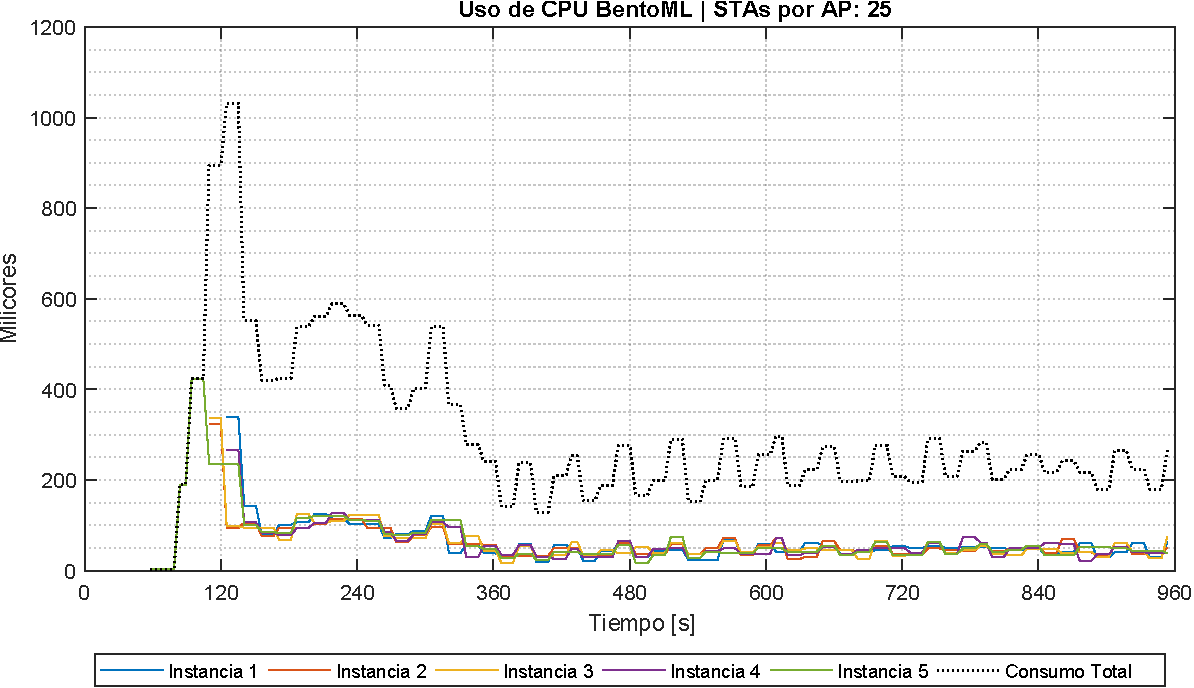
\includegraphics[width=\textwidth]{fig/08_datadriven/datadriven_11.pdf}
    \caption{Uso de CPU de BentoML con escalado automático para 25 STA por AP.}
    \label{fig:time_advance_consumption_stas25__ns_bentoml_datadriven}
\end{figure}

\subsection{Latencia de inferencia e ingestión de datos}

En esta subsección se evalúa la latencia media de inferencia del servicio BentoML y la latencia media de acceso a datos de InfluxDB. Ambas pruebas se realizan utilizando la herramienta de \textit{benchmarking} \texttt{hey}\footnote{\url{https://github.com/rakyll/hey}}, a través de un script personalizado que genera carga concurrente dirigida al servicio de inferencia de BentoML y a la interfaz de consulta de datos de InfluxDB.\\
\\
El objetivo es analizar el impacto del autoescalado en BentoML y la capacidad de respuesta de InfluxDB, proporcionando así una visión global del rendimiento del sistema bajo cargas de trabajo realistas. Para ello, se emiten solicitudes HTTP concurrentes, aumentando progresivamente el número de conexiones simultáneas de 1 a 100. Cada lote de solicitudes concurrentes, denotado como $C_n$, se considera una caso experimental independiente. Por ejemplo, fijar $C_n = 10$ implica el lanzamiento de 10 peticiones en paralelo que constituyen una ejecución experimental. Esta metodología es fundamental para garantizar la consistencia y fiabilidad estadística de los resultados; de lo contrario, mediciones fragmentadas o asincrónicas comprometerían su validez. Para cada prueba, se emiten $10 \times C_n$ solicitudes, donde $C_n \in \{1, \ldots, 100\}$. Tras cada lote, se establece un periodo de enfriamiento que permite al sistema retornar a su estado inactivo, específicamente, cuando BentoML opera con un único contenedor activo e InfluxDB presenta carga base. Cada escenario experimental se repite 25 veces, partiendo del contenedor del controlador Ryu (que normalmente desencadenaría dichos flujos de datos), manteniendo la topología de Mininet inactiva para eliminar interferencias. Los resultados promedio se muestran en las Figuras~\ref{fig:hey-inference-time-bento}, \ref{fig:hey-blocking-test-bento}, \ref{fig:hey-inference-time-influx} y \ref{fig:hey-blocking-test-influx}.

\begin{figure}[ht!]
    \centering
    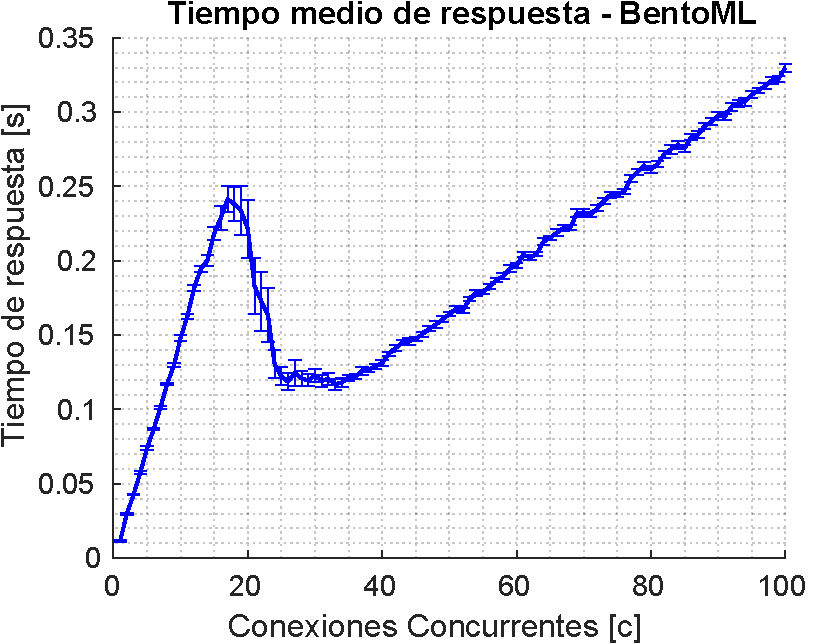
\includegraphics[width=0.65\textwidth]{fig/08_datadriven/datadriven_12.pdf}
    \caption{Tiempo medio de inferencia de BentoML en función de las solicitudes concurrentes.}
    \label{fig:hey-inference-time-bento}
\end{figure}

La Figura~\ref{fig:hey-inference-time-bento} presenta el tiempo medio de respuesta del servicio BentoML en función del número de solicitudes concurrentes. Se observa un incremento cuasi-lineal en el tiempo de respuesta, alcanzando una latencia máxima de aproximadamente 350 ms bajo 100 solicitudes concurrentes. La figura permite distinguir tres fases. En la fase inicial, de 0 a 15 solicitudes concurrentes, solo un contenedor permanece activo, lo que produce la pendiente más pronunciada de latencia. Este retraso activa la política de autoescalado, iniciando el despliegue de réplicas adicionales de BentoML. La fase intermedia, de 15 a 25 solicitudes, muestra un incremento continuado en el tiempo de respuesta, mientras el autoescalador añade progresivamente réplicas hasta alcanzar el límite superior de cinco. Más allá de las 25 solicitudes, en la fase final, el tiempo de respuesta continúa creciendo, pero a un ritmo significativamente menor, reflejando el balanceo de carga entre múltiples réplicas y la amortización del coste computacional.\\
\\
En contraste, la Figura~\ref{fig:hey-inference-time-influx} ilustra los resultados del mismo procedimiento experimental aplicado al servicio InfluxDB, enfocado en operaciones de lectura de la base de datos en lugar de tareas de inferencia. La latencia observada se mantiene notablemente estable a lo largo del experimento, con un máximo de aproximadamente 480 ms bajo condiciones de máxima concurrencia. Este comportamiento resulta especialmente destacable dado que InfluxDB no implementa mecanismos de autoescalado, una decisión de diseño orientada a preservar la consistencia de los datos. La figura revela una posible tendencia de crecimiento logarítmico en el tiempo de respuesta, lo cual indica un rendimiento escalable a pesar del aumento de carga.

\begin{figure}[ht!]
    \centering
    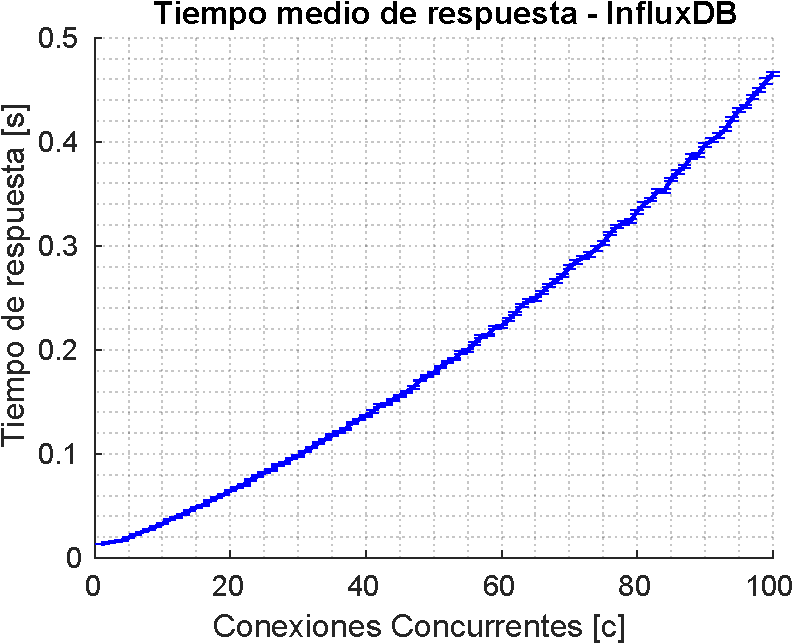
\includegraphics[width=0.6\textwidth]{fig/08_datadriven/datadriven_13.pdf}
    \caption{Tiempo medio de ingestión de datos en InfluxDB en función de las solicitudes concurrentes.}
    \label{fig:hey-inference-time-influx}
\end{figure}

Las dos figuras siguientes complementan el análisis previo incorporando los códigos de respuesta HTTP en la evaluación. Esta mejora permite identificar solicitudes exitosas y fallidas, considerando como fallo cualquier código de estado distinto de 200 OK. Además, este estudio integra restricciones de \gls{qos}, examinando cómo se comporta el sistema bajo diferentes umbrales máximos de tiempo de respuesta ($T_\text{max}$), específicamente entre 0.1 y 0.5 segundos. Para estimar la probabilidad de bloqueo ($P_b$) de cada servicio, se calcula la razón entre el número de solicitudes fallidas (aquellas con respuestas distintas de 200 o que superan el umbral $T_\text{max}$) y el número total de solicitudes. Los resultados para BentoML e InfluxDB se muestran en las Figuras~\ref{fig:hey-blocking-test-bento} y~\ref{fig:hey-blocking-test-influx}, respectivamente. En la Figura~\ref{fig:hey-blocking-test-bento}, cada curva ilustra la evolución de $P_b$ en función de la carga de solicitudes concurrentes bajo distintos niveles de \gls{qos}. El mecanismo de autoescalado de BentoML mitiga significativamente $P_b$ una vez que se despliega más de una réplica. Por ejemplo, con $T_\text{max} = 0.2$ s, $P_b$ desciende de 0.9 con 15 solicitudes concurrentes a menos de 0.02 cuando la carga se sitúa entre 25 y 40 solicitudes. Esto pone de manifiesto la eficacia del autoescalado para mantener la calidad del servicio ante una demanda creciente. Sin embargo, para umbrales de \gls{qos} más estrictos ($T_\text{max} = 0.1$ s), incluso cargas moderadas conducen a probabilidades de bloqueo elevadas, debido principalmente a la sobrecarga adicional introducida por el balanceador de carga dinámico y al tiempo computacional inherente requerido por cada inferencia, que, como se mostró anteriormente, puede alcanzar hasta 0.05 s incluso bajo cargas mínimas.

\begin{figure}[ht!]
    \centering
    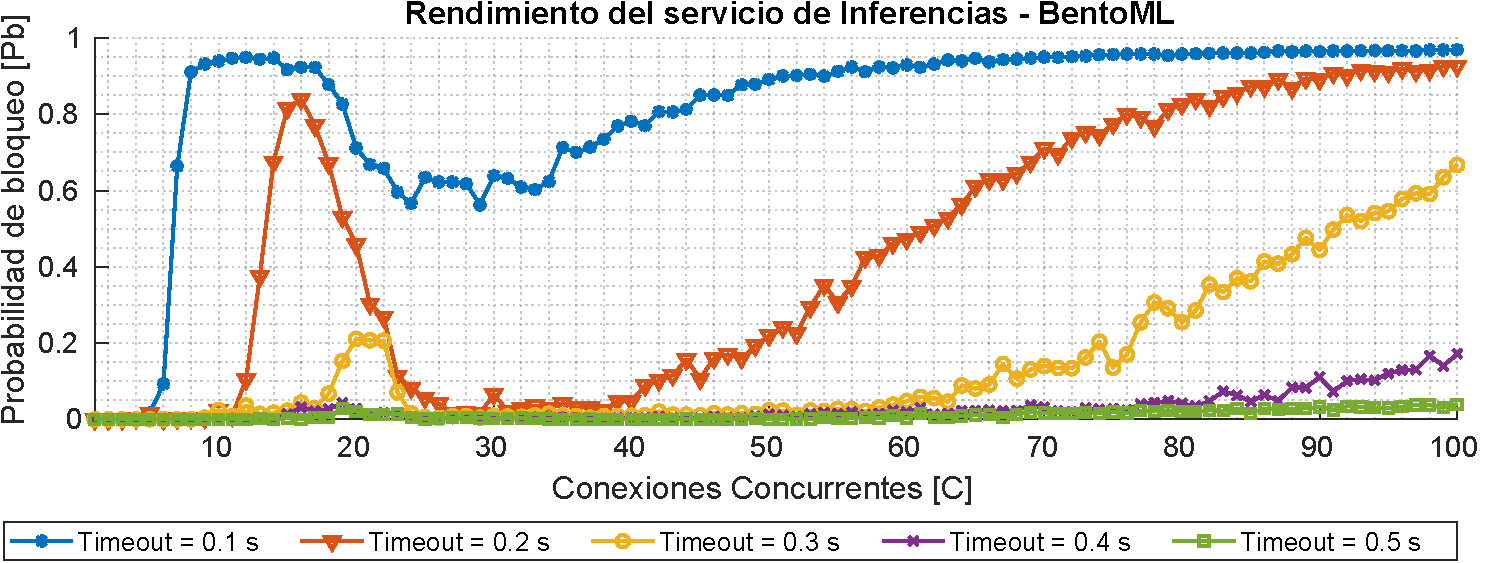
\includegraphics[width=0.9\textwidth]{fig/08_datadriven/datadriven_14.pdf}
    \caption{Probabilidad de bloqueo en BentoML bajo distintos umbrales de \gls{qos}.}
    \label{fig:hey-blocking-test-bento}
\end{figure}

\begin{figure}[ht!]
    \centering
    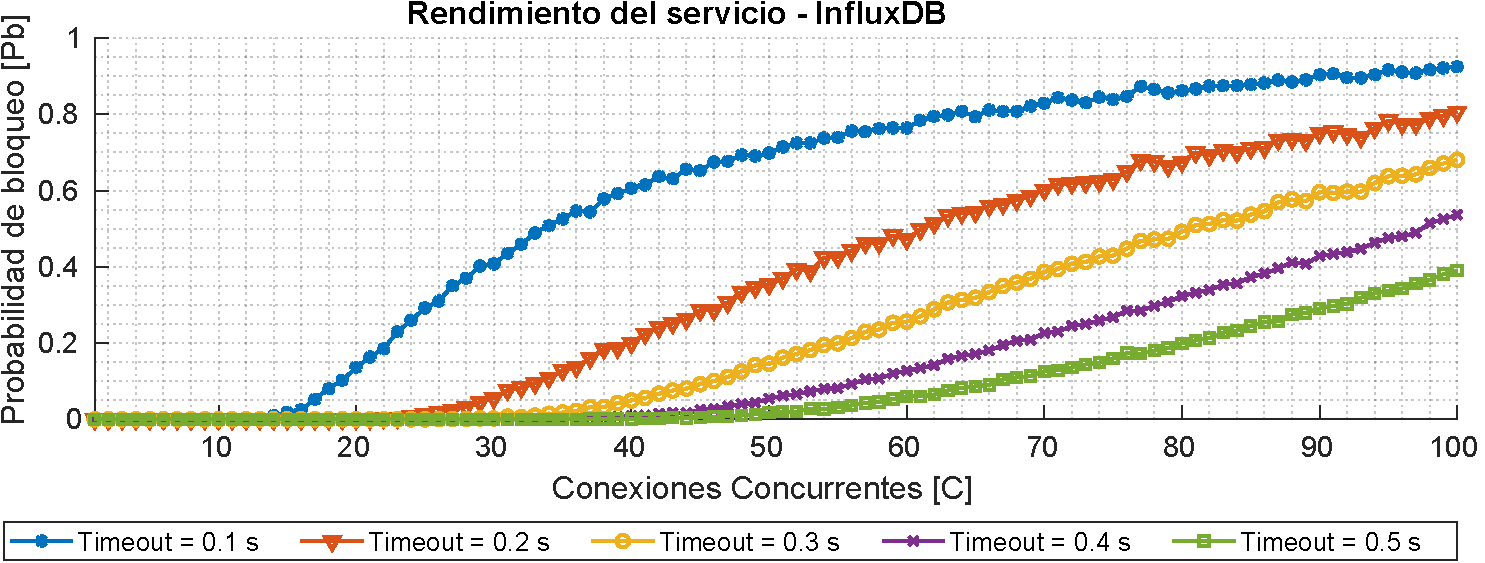
\includegraphics[width=0.9\textwidth]{fig/08_datadriven/datadriven_15.pdf}
    \caption{Probabilidad de bloqueo en InfluxDB bajo distintos umbrales de \gls{qos}.}
    \label{fig:hey-blocking-test-influx}
\end{figure}

En contraste, la Figura~\ref{fig:hey-blocking-test-influx} presenta el análisis de la probabilidad de bloqueo para el servicio InfluxDB. En este caso, el comportamiento es más predecible y menos sensible a las variaciones de carga. Aunque no se emplea un mecanismo de autoescalado, la base de datos mantiene un rendimiento relativamente estable, y su probabilidad de bloqueo aumenta de forma gradual con la carga. Esto confirma la robustez de InfluxDB frente a cargas de consulta moderadas incluso en ausencia de escalabilidad elástica.


\subsection{Estimación del tiempo promedio de reconfiguración de red}

Esta subsección presenta la estimación del tiempo promedio requerido para completar un ciclo de reconfiguración en la arquitectura propuesta. El proceso de reconfiguración es desencadenado por el controlador \gls{sdn}, implementado con el framework Ryu, el cual reacciona ante comportamientos anómalos detectados en la red de sensores \gls{iiot}. Para cuantificar el tiempo de reconfiguración, se descompone el proceso en sus dos componentes principales: (i) el tiempo necesario para que Ryu acceda y recupere los datos de los sensores desde la base de datos de series temporales InfluxDB, y (ii) el tiempo requerido para enviar dichos datos al servicio de inferencia en la nube desplegado mediante BentoML y obtener un resultado de clasificación. Dado que ambos intercambios de comunicación (Ryu $\rightarrow$ InfluxDB y Ryu $\rightarrow$ BentoML) han sido previamente caracterizados en términos de sus tiempos de respuesta promedio bajo cargas concurrentes, se define el tiempo medio de reconfiguración, denotado $T_{reconf}$, como:

\begin{equation}
T_{reconf} = T_{read}^{Influx} + T_{infer}^{Bento}
\end{equation}

donde $T_{read}^{Influx}$ representa el tiempo promedio requerido para recuperar las lecturas más recientes de los sensores en InfluxDB, y $T_{infer}^{Bento}$ denota el tiempo promedio de inferencia del servicio BentoML. Estas dos operaciones encapsulan las latencias dominantes en el bucle de reconfiguración. \\
\\
Aunque se produce una etapa adicional de procesamiento dentro del controlador Ryu, responsable de componer la solicitud al servicio de inferencia e interpretar el resultado devuelto, este esfuerzo computacional local implica un número mínimo de operaciones en Python (p.~ej., análisis sintáctico, verificación de condiciones), y su tiempo de ejecución resulta despreciable en comparación con la sobrecarga de comunicación en red y de inferencia. Esta consideración es aún más válida a medida que aumenta el número de estaciones \gls{iiot}, dado que las operaciones locales no escalan de forma proporcional al número de sensores. Por tanto, la estimación de $T_{reconf}$ constituye una cota superior realista del tiempo promedio necesario para detectar una anomalía e iniciar una política de reconfiguración en la red, permitiendo una gestión receptiva y escalable en entornos industriales dinámicos.

\section{Conclusiones}

Este trabajo ha presentado una arquitectura novedosa, totalmente contenerizada, que combina recursos en el \textit{edge} y en el \textit{cloud} para habilitar una toma de decisiones adaptativa y basada en datos en entornos de \gls{iiot}. La arquitectura propuesta aborda limitaciones críticas identificadas en el estado del arte, tales como la ausencia de integración extremo a extremo a lo largo del continuo \gls{iiot}-\textit{edge}-\textit{cloud}, la falta de mecanismos de reconfiguración dinámica basados en analítica en línea, y la limitada escalabilidad y preparación para despliegue de los prototipos existentes.\\
\\
A través de una evaluación experimental exhaustiva, se han obtenido varios hallazgos clave. En primer lugar, el sistema demuestra capacidades de despliegue rápido, alcanzando plena operatividad en menos de cinco minutos. En segundo lugar, la arquitectura exhibe un uso estable y eficiente de los recursos, con patrones predecibles de consumo de memoria y CPU en los distintos microservicios.  Cabe destacar que el servicio de inferencia basado en BentoML se beneficia significativamente de la autoescalabilidad horizontal, manteniendo tiempos de respuesta bajos incluso bajo altas cargas de peticiones concurrentes. Asimismo, InfluxDB asegura un acceso a los datos de baja latencia en todos los experimentos, lo que confirma su idoneidad para tareas de monitorización continua en escenarios \gls{iiot}. Con ello, es posible estimar el tiempo promedio de reconfiguración de red, obtenido a partir de la combinación de los tiempos de acceso a la base de datos y de respuesta del servicio de inferencia. Los resultados indican que el sistema es capaz de sostener ciclos de reconfiguración inferiores al segundo, lo cual resulta esencial para la adaptación en tiempo real en despliegues industriales. Además, el análisis de la probabilidad de bloqueo bajo distintos umbrales de \gls{qos} pone de manifiesto las ventajas del escalado elástico, ya que reduce sustancialmente la probabilidad de degradación del servicio bajo condiciones de carga elevada.\\
\\
Más allá de su validación técnica, este trabajo introduce una arquitectura disruptiva que cubre vacíos existentes en la literatura al integrar inferencia, telemetría y control \gls{sdn} en un marco unificado y reproducible, liberando todo el sistema y los conjuntos de datos como \textit{opensource}. En consecuencia, la arquitectura propuesta no solo constituye una contribución científica, sino que también sienta las bases para el desarrollo de soluciones industriales más resilientes, flexibles y adaptativas, capaces de responder a las crecientes demandas de digitalización y autonomía en la industria 4.0. 
